\capitolo{Pianificazione del Moto}
Pianificazione del moto significa scegliere la legge di moto, ossia \textit{La relazione matematica che esprime il moto in termini di posizione, velocità e accelerazione di un asse, motore o carico, in funzione di un parametro indipendente.}
\begin{itemize}
    \item Tempo, \(t [s]\)
    \item Posizione di un altro asse, \(q [m]\)
    \begin{itemize}
        \item Virtuale: camme elettroniche come clock di macchine
        \item Reale
        \begin{itemize}
            \item 2 assi meccanicamente accoppiati: camme meccaniche
            \item 2 assi accoppiati solo con controllo: camme elettriche
        \end{itemize}
    \end{itemize}
\end{itemize}

\paragrafo{Scelta delle Leggi di Moto}
Le specifiche in termini di legge di moto sono tendenzialmente poche, legate a: tempo di ciclo, spazio percorso, velocità minima, massima; a partire dalle quali va fatta una ottimizzazione consci di non poter ottenere una legge di moto perfetta.

\sottoparagrafo{Criteri di Scelta}
La scelta del tipo di legge di moto viene effettuata a partire da alcune caratteristiche progettuali:
\begin{enumerate}
    \item Minimizzazione di velocità massima o RMS
    \item Minimizzazione di accelerazione massima o RMS
    \item Minimizzazione dell'energia
    \item Minimizzazione della potenza
    \item Garantire realizzabilità della legge di moto in termini dinamici\footnote{In termini di banda passante di motore, controllo, di spettro della legge di moto e vibrazioni.}
\end{enumerate}
In generale la scelta dipende da progetto a progetto, tuttavia conviene cercare di avere focus su un parametro in particolare, perché diversi di questi risultano tra loro in trade off. Per esempio scegliere una forma d'onda di velocità triangolare senza riposi limita l'accelerazione massima al valore RMS, tuttavia questo potrebbe non permettere una buona scelta del motore per il quale non si andrebbe ad utilizzare la zona di lavoro intermittente.

\sezione{Formulazione delle principali leggi di Moto}
Le leggi di moto si dividono in due categorie: Punto-Punto (PP), quando le specifiche sono su punto di inizio e fine o Con specifiche su punti o tratti intermedi.
All'interno della tipologia Punto-Punto c'è un sottogruppo per cui la velocità inziale e finale sono nulle detto Rest-to-Rest (RtR).
In seguito verranno analizzati alcune leggi di moto del caso PP, con particolare attenzione ai sottocasi RtR.

Di particolare interesse è il moto simmetrico, ossia avente funzione velocità simmetrica rispetto \(\frac{T}{2}\).

\sottosezione{Parametrizzazione}
Per successive analisi conviene introdurre una normalizzazione dei tempi di accelerazione \(\lambda_A = \frac{t_A}{T}\) e decelerazione \(\lambda_D = \frac{t_D}{T}\), tenendo conto che per ciascuno vale \(0 < \lambda < 1\) e \(0 < \lambda_A + \lambda_D < 1\).

\paragrafo{Parametri di merito:}
A partire dalla parametrizzazione si possono ricavare per i vari parametri di progetto dei valori indipendenti da \(h\) alzata e \(T\) periodo di lavoro.
L'utilizzo di questi valori permette di semplificare la scelta della legge di modo fornendo delle figure di merito confrontabili, da porter tabellare.
\begin{itemize}
    \item \(C_V\) coefficiente di velocità massima, con velocità massima \(v_{max}=\frac{h}{T}C_V\)
    \item \(C_{A+}\) coefficiente di accelerazione massima, con accelerazione massima \(a_{max}=\frac{h}{T^2}C_{A+}\)
    \item \(C_{A-}\) coefficiente di decelerazione massima, con decelerazione massima \(a_{min}=\frac{h}{T^2}C_{A-}\)
    \item \(C_A^{RMS}\) coefficiente di accelerazione RMS, con accelerazione RMS \(a^{RMS}=\frac{h}{T^2}C_A^{RMS}\)
    \item \(C_J\) coefficiente di jerk massimo, con jerk massimo \(j_{max}=\frac{h}{T^3}C_J\)
\end{itemize}
Per poter ricavare dei valori generici è sufficiente ricavare la grandezza di cui interessa il coefficiente, considerando un alzata di 1 metro in un periodo di 1 secondo.

\sottosezione{Scalatura delle leggi}
A partire dalle leggi di moto utilizzate è possibile scalarle in relazione alle richieste della specifica applicazione.
Guardando velocità, accelerazioni, jerk massimi e accelerazione RMS, si può cogliere come la variazione di alzata \(h\) provoca una variazione lineare del coefficiente (raddoppiare l'alzata porta a raddoppiare il coefficiente).
Mentre la variazione del tempo dipende in modo inversamente proporzionale con grado pari all'ordine della derivata in esame (dimezzare il tempo porta a raddoppiare la velocità, ma a quadruplicare le accelerazioni).

\sottosezione{Rampa di posizione}
Una rampa (limitata) di posizione è una legge di moto che descrive una funzione continua, ma non derivabile\footnote{Nel senso che la derivata destra e sinistra non coincidono in corrispondenza di punti di inizio e fine della rampa. Si considerano in seguito la velocità e l'accelerazioni come funzioni derivate da funzione definita a tratti.}; da questa legge di posizione si ottiene una velocità discontinua e accelerazione che tende all'infinito, cosa tuttavia irrealizzabile, perché richiederebbe motore a coppia infinita.

\sottosezione{Trapezoidale in velocità}
Una forma trapeziodale in velocità risulta in una funzione posizione continua e derivabile, di velocità continua ma non derivabile, quindi accelerazione discontinua, ma finita.
Nel caso di traiettoria RtR \( v_{fin} = 0 = \int^{t_{fin}}_{t_{in}} \acc{q} dt \), ossia le aree sottese dalla funzione accelerazione devono essere uguali.

\begin{figure}[h]
    \centering
    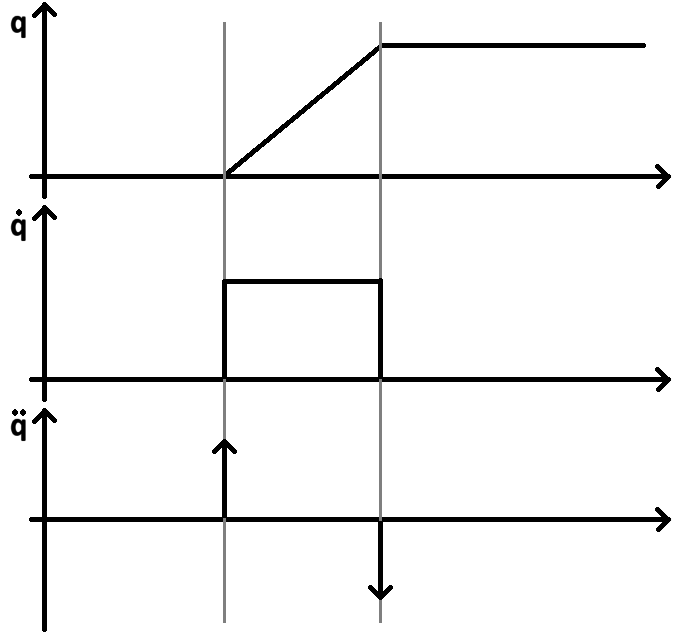
\includegraphics[width=0.3\textwidth]{Immagini/rampa_pos.png}
    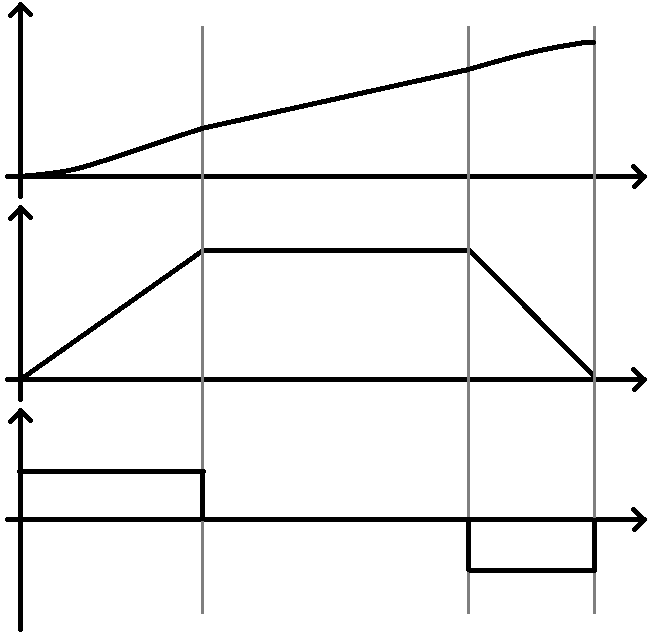
\includegraphics[width=0.3\textwidth]{Immagini/trapezoidale_vel.png}
    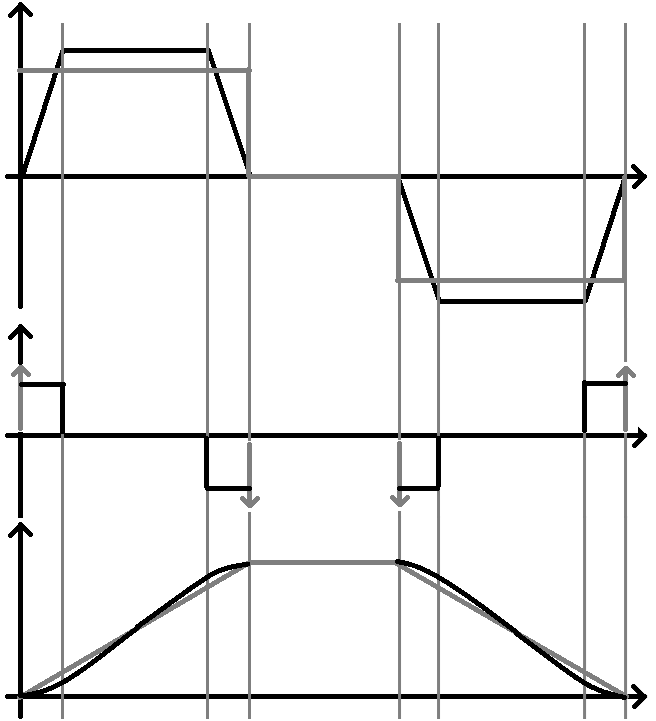
\includegraphics[width=0.3\textwidth]{Immagini/trapezoidale_acc.png}
    \caption{Rampa Posizione sx; Trapeziodale Velocità centro; Trapezoidale Accelerazione dx}
\end{figure}

\sottosottosezione{Grandezze significative (RtR)}
La velocità massima ottenibile si può determinare integrando la funzione di velocità, o più semplicemente facendo valutazioni geometriche sul trapezio, da cui si ottiene \(V_{max} = \frac{h}{\frac{t_A}{2}+t_C +\frac{t_D}{2}}\).
Possono essere ricavate di conseguenza l'accelerazione \(\abs{A} = \frac{V_{max}}{t_A}\) e la delecelazione \(\abs{D} = \frac{V_{max}}{t_D}\). Vale inoltre \(\frac{\abs{A}}{\abs{D}} = \frac{t_D}{t_A}\).

\paragrafo{Velocità con parametrizzazione:}
La velocità massima ottenibile diventa \(V_{max} = \frac{h}{T} \frac{1}{1-\frac{\lambda_A}{2}-\frac{\lambda_D}{2}}\), dove \(v_{media} = \frac{h}{T}\) ed è indipendente dalla traiettoria, viene definito \(C_v = \frac{1}{1-\frac{\lambda_A}{2}-\frac{\lambda_D}{2}}\).

\paragrafo{Accelerazione con parametrizzazione:}
L'accelerazione ottenuta diventa \(A=\frac{h}{T^2} \frac{1}{\lambda_A}\frac{1}{1-\frac{\left(\lambda_A + \lambda_D \right)}{2}}\), dove \(a = \frac{h}{T^2}\) rappresenta l'equivalente valore in caso di moto con accelerazione costante, da cui viene definito \(C_{A+} = \frac{1}{\lambda_A}\frac{1}{1-\frac{\left(\lambda_A + \lambda_D \right)}{2}}\).
In modo del tutto simile, associata alla decelerazione \(D\), viene definito \(C_{A-} = \frac{1}{\lambda_D}\frac{1}{1-\frac{\left(\lambda_A + \lambda_D \right)}{2}}\).

\paragrafo{Accelerazione RMS:}
L'accelerazione RMS si ottiene calcolando l'integrale usando le valutazioni geometriche per l'accelerazione e ricordando il legame tra \(\abs{D}\) e \(\abs{A}\), da cui si può ricavare l'espressione finale \(\acc{q}^{RMS} = \frac{h}{T^2} C_A \sqrt{\lambda_A + \frac{\lambda_A^2}{\lambda_D}}\), in cui viene definito \(C_A^{RMS} = C_A \sqrt{\lambda_A + \frac{\lambda_A^2}{\lambda_D}}\).
Analizzando la funzione si otttiene un minimo assoluto per \(\lambda_A=\lambda_D =\frac{1}{3}\), valori in corrispondenza dei quali si ottiene un moto simmetrico (equamente distribuito tra accelerazione, velocità costante e decelerazione).

\paragrafo{Potenza meccanica:}
Nel moto trapezoidale in velocità i punti più critici in termini di velocità sono per termine di fase di accelerazione e inizio fase di decelerazione, per cui si hanno \(\max{\acc{q}}\) e \(\max{\dot{q}}\), che portano ad avere, nel caso inerziale, \(\max{W_M}\) proporzionale a \(\max{\acc{q}} \cdot \max{\dot{q}}\).
A partire dalla potenza massima, si può definire il coefficiente di potenza massima come \(C_W = C_V C_A = \frac{1}{\lambda(1-\lambda)(1-\lambda)}\) nel caso di moto simmetrico.

\sottosottosezione{Legge trapezoidale con moto simmetrico, RtR}
Nel caso di legge trapezoidale con moto simmetrico, vale \(\lambda_A=\lambda_D := \lambda \in (0,1/2]\), i coefficienti diventano: \(C_V = \frac{1}{1-\lambda}\); \(C_A = \frac{1}{\lambda}\frac{1}{1-\lambda}\); \(C_A^{RMS} = C_A \sqrt{2\lambda}\).

\begin{figure}[h]
    \centering
    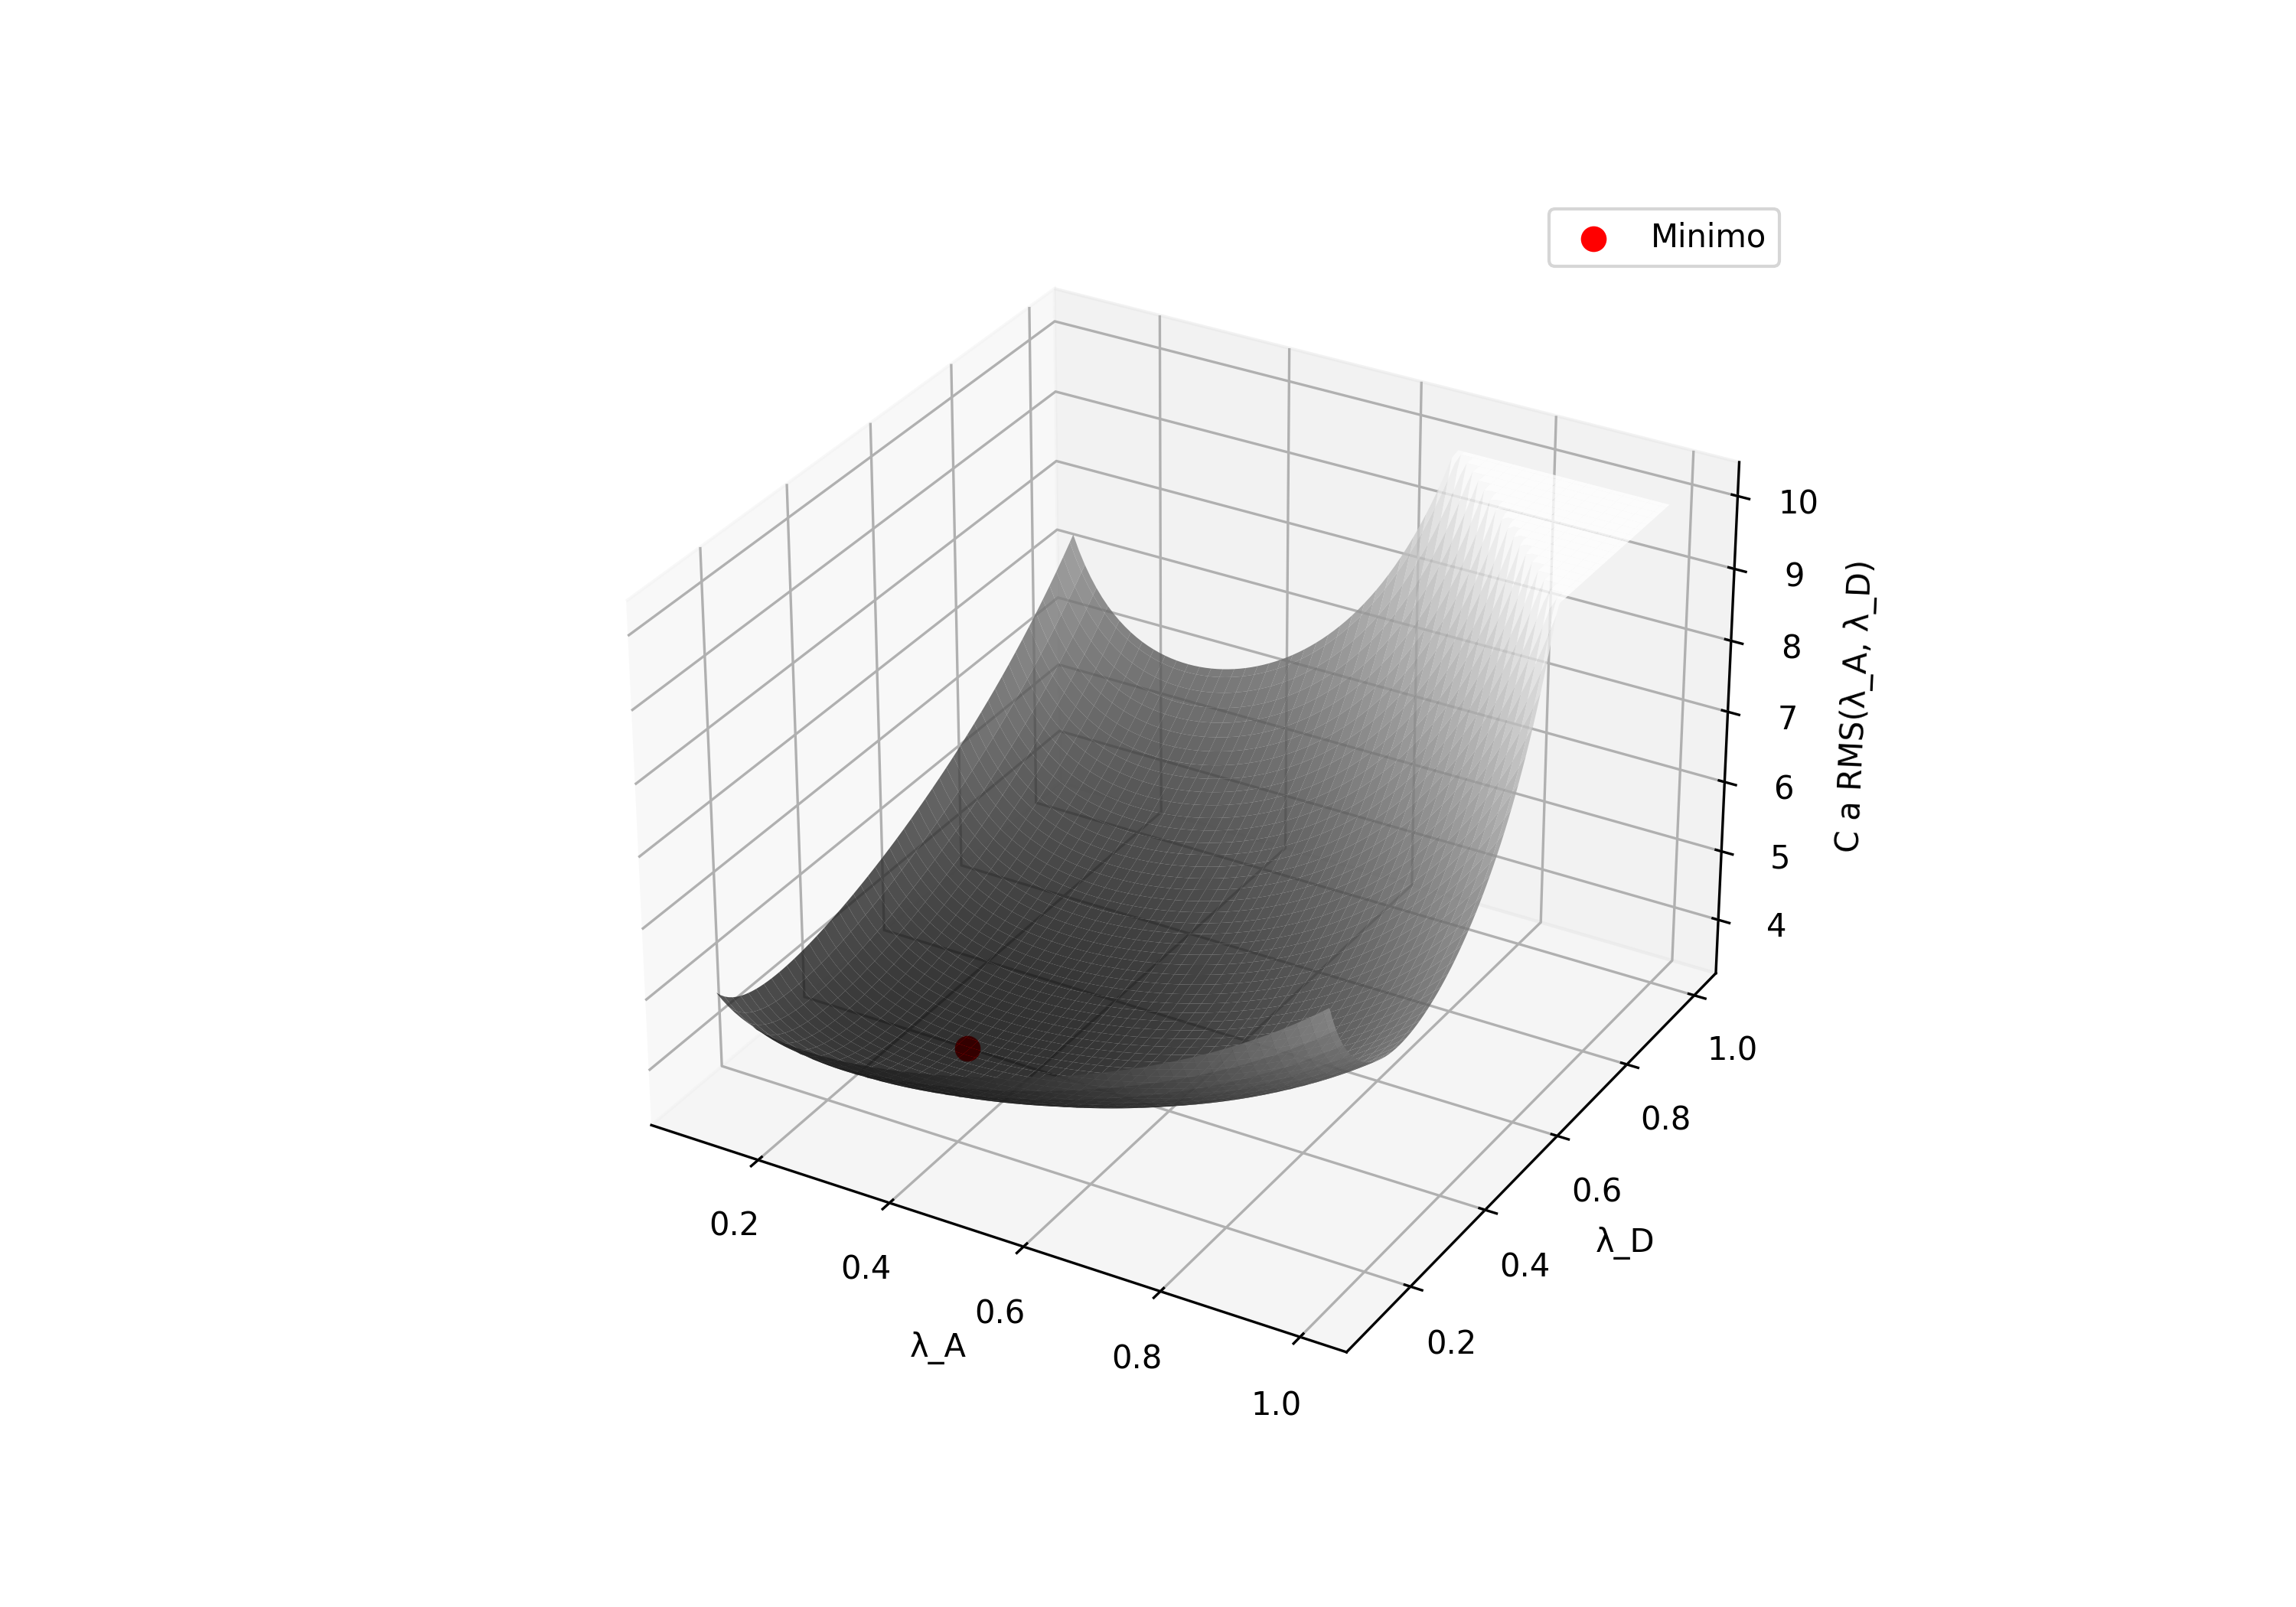
\includegraphics[width=0.4\textwidth]{Immagini/CaRMS.png}
    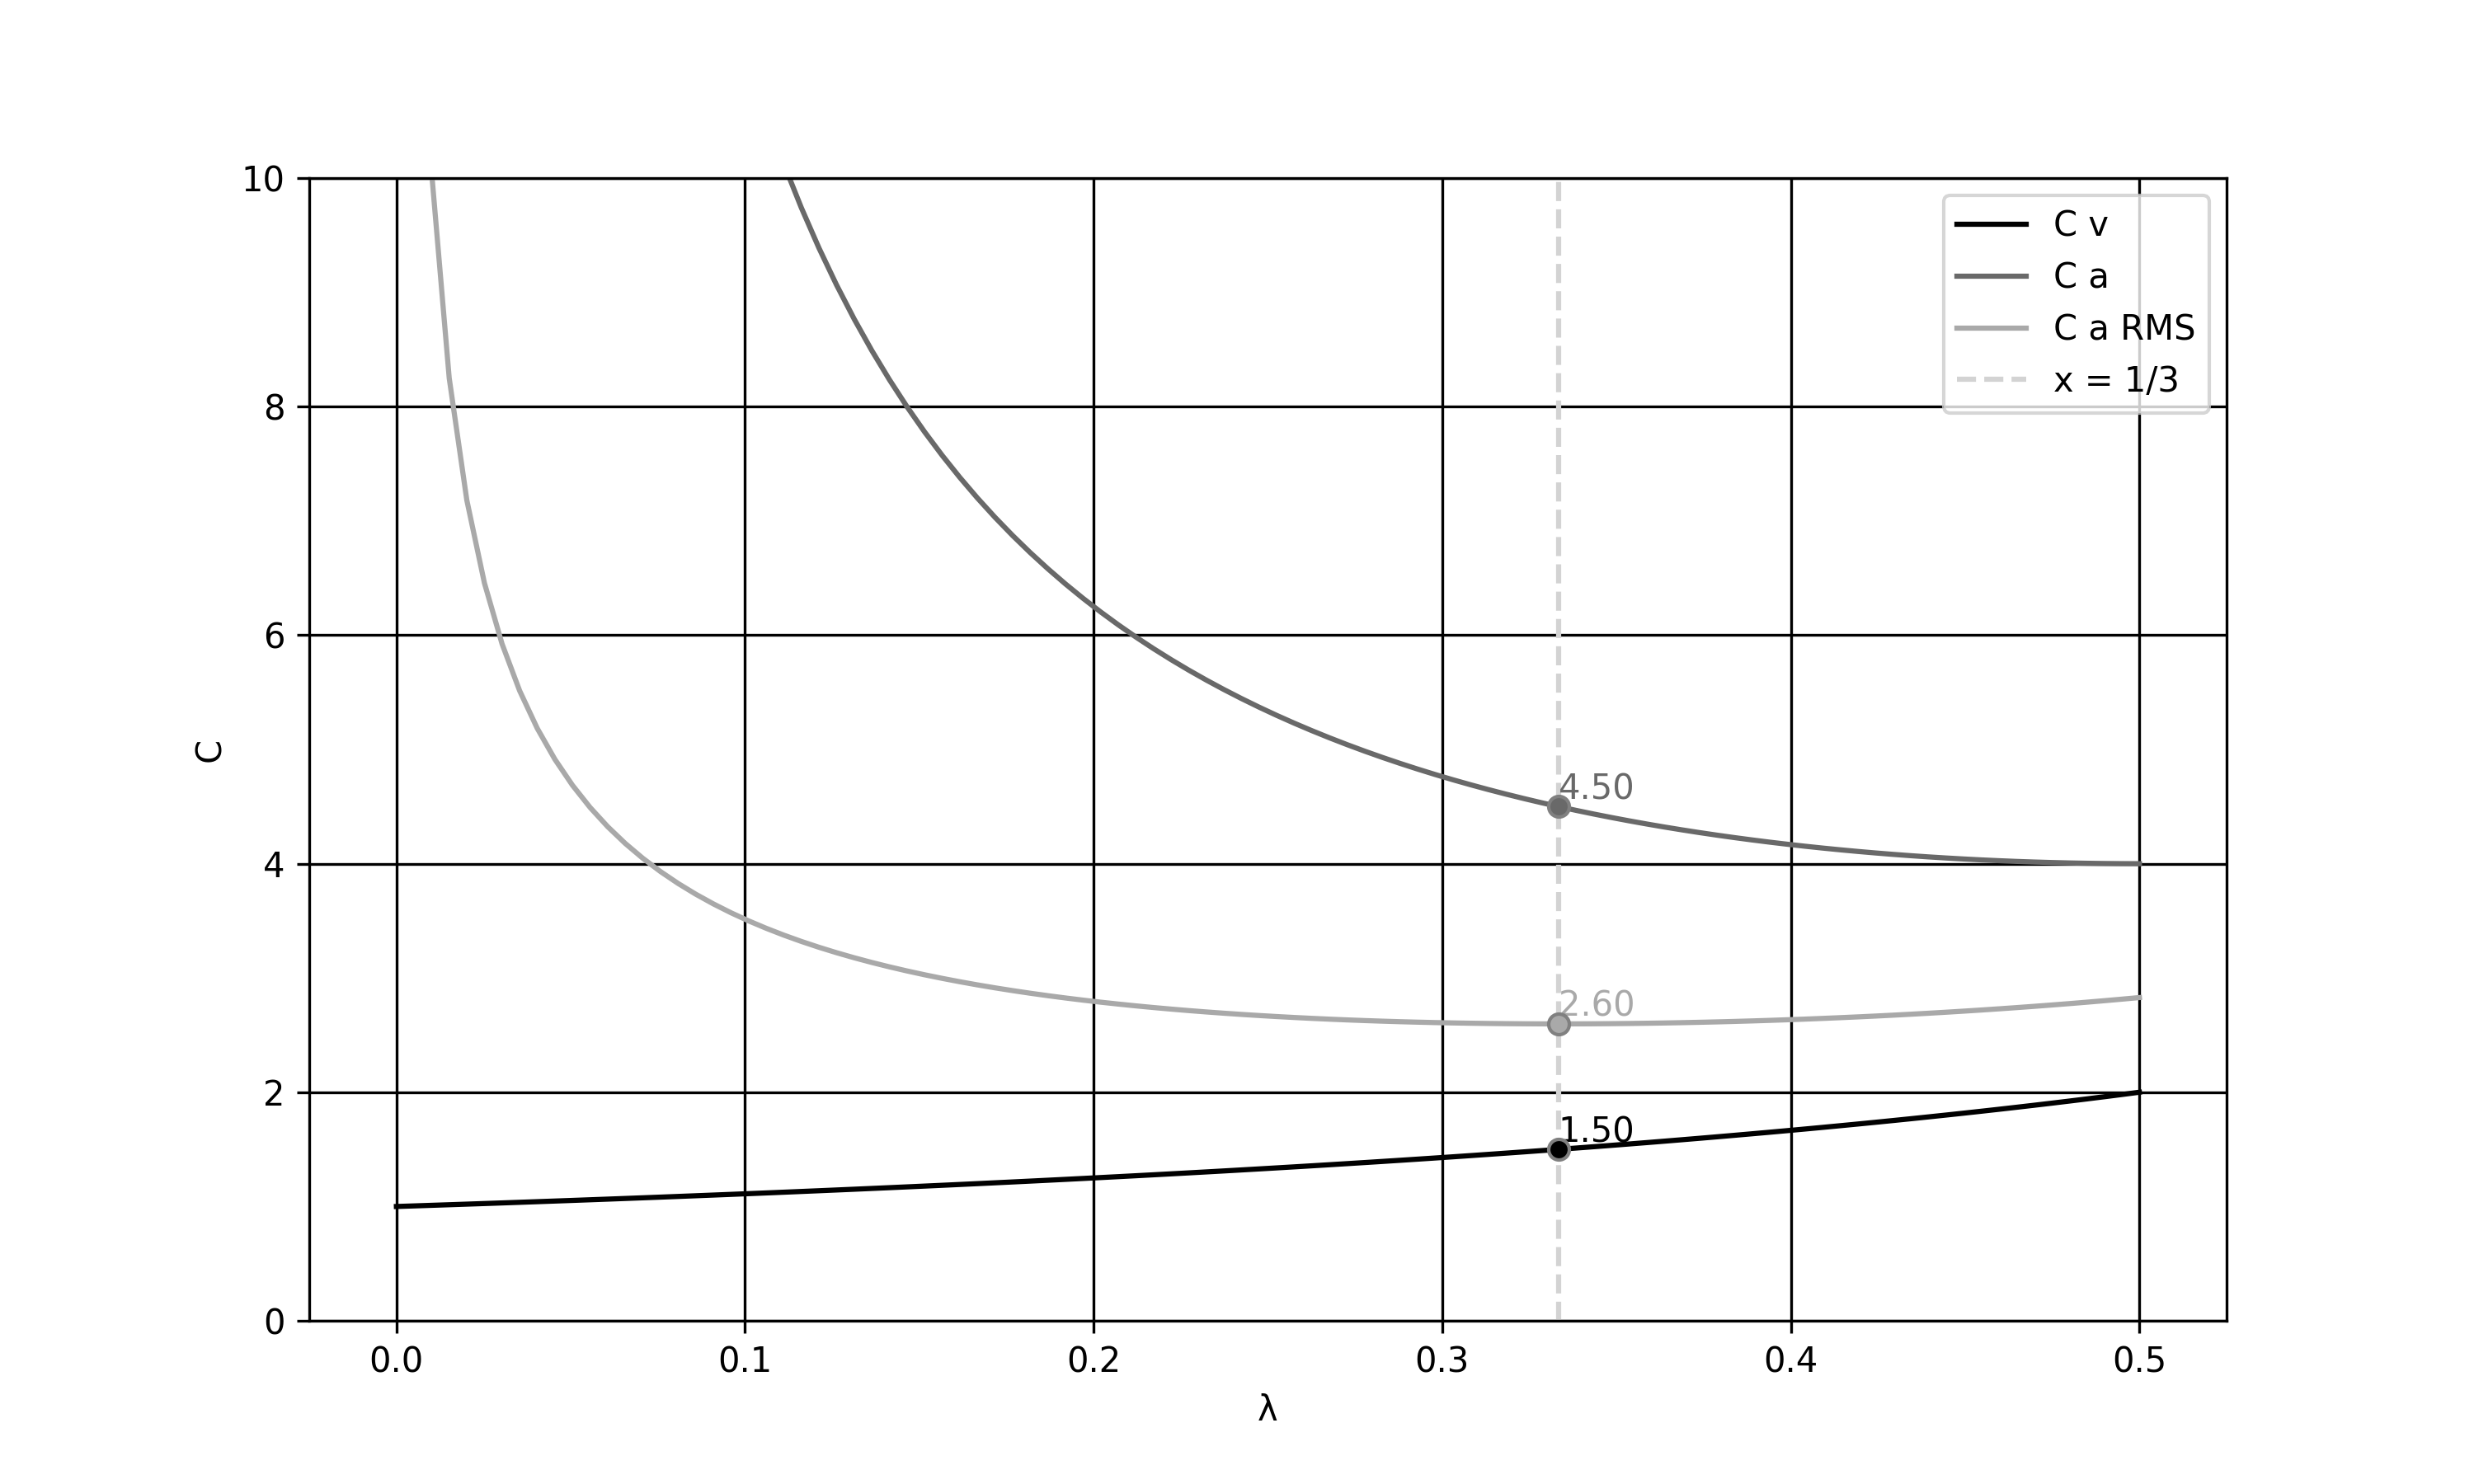
\includegraphics[width=0.55\textwidth]{Immagini/CvCaCaRMS.png}
    \caption{Coeff accelerazione RMS sx; Coeff per caso moto simmetrico dx}
\end{figure}

In questo caso risulta chiaro come ci sia un trade-off tra velocità e accelerazione.
Una prima scelta sensata (da cui partire per poi affinare la ricerca) potrebbe essere \(\lambda = \frac{1}{3}\), valore per cui si ha il minimo di coefficiente di accelerazione RMS, un basso coefficiente di accelerazione e un valore abbastanza basso di coefficiente di velocità, infine è anche prossimo all'ottimo energetico.

\paragrafo{Simmetria vs Assimetria:}
Quando c'è una disparità tra forze esterne in accelerazione e decelerazione (es ascensore o piano inclinato), conviene utilizzare una legge assimetrica al posto di una simmetrica per distribuire meglio le due aree.
In modo del tutto equivalente si può utilizzare l'espressione ottenuta per il caso simmetrico anche per il caso asimmetrico introducendo un \(\lambda_m=\frac{\lambda_A+\lambda_B}{2}\).

\sottosezione{Trapezoidale in Accelerazione}
A partire da una legge trapezoidale in velocità, considero di fare una legge trapezoidale in accelerazione che abbia la stessa velocità massima, questo influenza la scelta dei raccordi\footnote{Nel caso in figura i raccordi sono lineari, tuttavia potrebbero essere polinomiali, esponenziali, sinusoidali, ecc nel caso debbano essere modificati i coefficienti o migliorato lo spettro della legge di moto.}.
Infatti per ottenere la stessa velocità massima le aree delle due accelerazione deve essere uguale; a seguito di semplici valutazioni geometriche si può ricavare l'accelerazione massima per la trapezoidale in accelerazione come \(A_m=\frac{h}{T^2}\frac{1}{\lambda(1-\lambda)(1-\gamma)}\), dove \(\gamma = \frac{t_R}{t_A}\) ossia il tempo di raccordo normalizzato al tempo totale di accelerazione. 
In questa legge di moto l'accelerazione risulta continua, cosa che aumenta la semplicità realizzativa, vengono ridotte le vibrazioni, ma aumentano l'accelerazione massima e RMS.


\sottosottosezione{Jerk}
Il jerk è la derivata nel tempo dell'accelerazione. Un jerk finito porta ad avere accelerazione continua, si parla in questi casi di legge di moto dolci; un jerk infinito porta ad avere un'accelerazione discontinua, si parla quindi di leggi non dolci.
Anche per il jerk si può definire il coefficiente di jerk massimo \(\dddot{q} = \frac{h}{T^3}C_J\).
Nel caso di trapezoidale in accelerazione \(C_J = \frac{C_A}{\lambda \gamma}\)

\sottosezione{Polinomiale di Terzo Grado}
Si parla in generela di polinomiale per intendere una funzione polinomiale in posizione di un certo ordine.

Nel caso di terzo grado la legge di moto è definita dalle seguenti equazioni.
\[\begin{cases}
    q(t) = a_0 + a_1 (t-t_0) + a_2 (t-t_0)^2 + a_3 (t-t_0)^3 \\
    \dot{q}(t) = a_1 + 2 a_2 (t-t_0) + 3 a_3 (t-t_0)^2 \\
    \Ddot{q}(t) = 2 a_2 + 6 a_3 (t-t_0)
\end{cases}\]

Per definire univocamente il polinomio sono necessarie 4 condizioni, che solitamente sono:
\[\begin{cases}
    q(t_0) = q_{in}  \\
    q(t_0+T) = q_{fine}  \\
    \dot{q}(t_0) = \dot{q}_{in}  \\
    \dot{q}(t_0+T) = \dot{q}_{fine}  
\end{cases}\]
E a partire dalle quali è possibile ottenere i coefficienti \(a_0,a_1,a_2,a_3\).

Nel caso di polinomiale di terzo grado avente \(h=1, \ T=1, \ t_0=0\) le espressioni della legge di moto, per \(t\in[0,T]\), diventano:
\[\begin{cases}
    q(t) = 3 t^2 - 2 t^3 \\
    \dot{q}(t) = 6 t + 6 t^2 \\
    \Ddot{q}(t) = 6 - 12 t \\
    \dddot{q}(t) \neq -12 \ !!!
\end{cases}\]

Prestare estrema attenzione al calcolo del jerk, perchè per leggerezza si potrebbe scrivere \(\dddot{q}(t) = -12\), tuttavia sarebbe scorretto, perché nei punti di estremo la velocità non è nulla, ciò significa che le tangenti destra e sinistra sono diverse, per quei valori il jerk è infinito.

Per quanto riguarda i coefficienti tenere da conto che la polinomiale di terzo grado ha il valore minimo per quanto riguarda i coefficienti di accelerazione RMS di tutte le leggi di moto classiche. I valori sono: \(C_V=1.5, \ C_A = 6, \ C_A^{RMS}=3.4, \ C_J = \infty\)


\sottosezione{Polinomiale di Quinto Grado}
La polinomiale di quinto grado utilizza 6 coefficienti, quindi il problema per essere ben posto richiede 6 condizioni al contorno. In modo del tutto simile al caso della polinomiale di terzo grado in generale sono \(q_{in} \ q_{fine} \ \dot{q}_{in}, \ \dot{q}_{fine}, \ \Ddot{q}_{in}, \ \Ddot{q}_{fine}\).
Posizione, velocità sono continue e derivabili, l'accelerazione è solo continua, il jerk è finito ma discontinuo.

Considerando la condizione RtR e usando la normalizzazione, considero gli step di creazione dei grafici:
\begin{enumerate}
    \item Punti per velocità e accelerazioni nulle
    \item Determinazione massimo velocità in \(t=1/2\)
    \item Tracciamento della velocità
    \item Valutazioni sulle tangenti di accelerazione agli istanti iniziali e finali: per un polinomio di terzo grado\footnote{Che è quello che si ottiene in accelerazione, avendo derivato due volte un polinomio di quinto grado.} ci sono 2 punti a tangente nulla e devono essere in corrispondenza dei valori di massimo e minimo\footnote{Non è possibile porre a tangenti nulle i valori iniziali e finali perché altrimenti l'accelerazione dovrebbe rimanere costante. {\color{red}(verificare l'affermazione)}}
    \item Tracciamento dell'accelerazione
    \item Tracciamento del jerk a partire da punti notevoli dell'accelerazione e soprattutto valutazioni su punti di discontinuità presenti nei punti iniziali e finali (legate a considerazione su accelerazione di cui sopra)
    \item Tracciamento della posizione prestando attenzione alle tangenti nulle iniziali e finali.
\end{enumerate}

\sottosezione{Polinomiale di Settimo Grado}
Nel polinomio di settimo grado i coefficienti sono 8 e quindi le condizioni da imporre sono 8.
In questo caso posizione, velocità, accelerazione sono continue e derivabili, il jerk è continuo ma non derivabile.

\paragrafo{Grado Terzo vs Quinto, Settimo:}
Esaminando la tabella dei coefficienti e in particolare confrontando il polinomio di quinto e settimo grado con quello di terzo grado si può notare come la miglior dolcezza venga ripagata con un peggioramento dei coefficienti di velocità e accelerazione.
Questo perché il maggior numero di radici può portare ad avere punti di massimo e minimo all'interno dell'intervallo temporale in esame, peggiorando drasticamente tutte le caratteristiche di velocità, accelerazione e consumo energetico.

\begin{figure}[h]
    \centering
    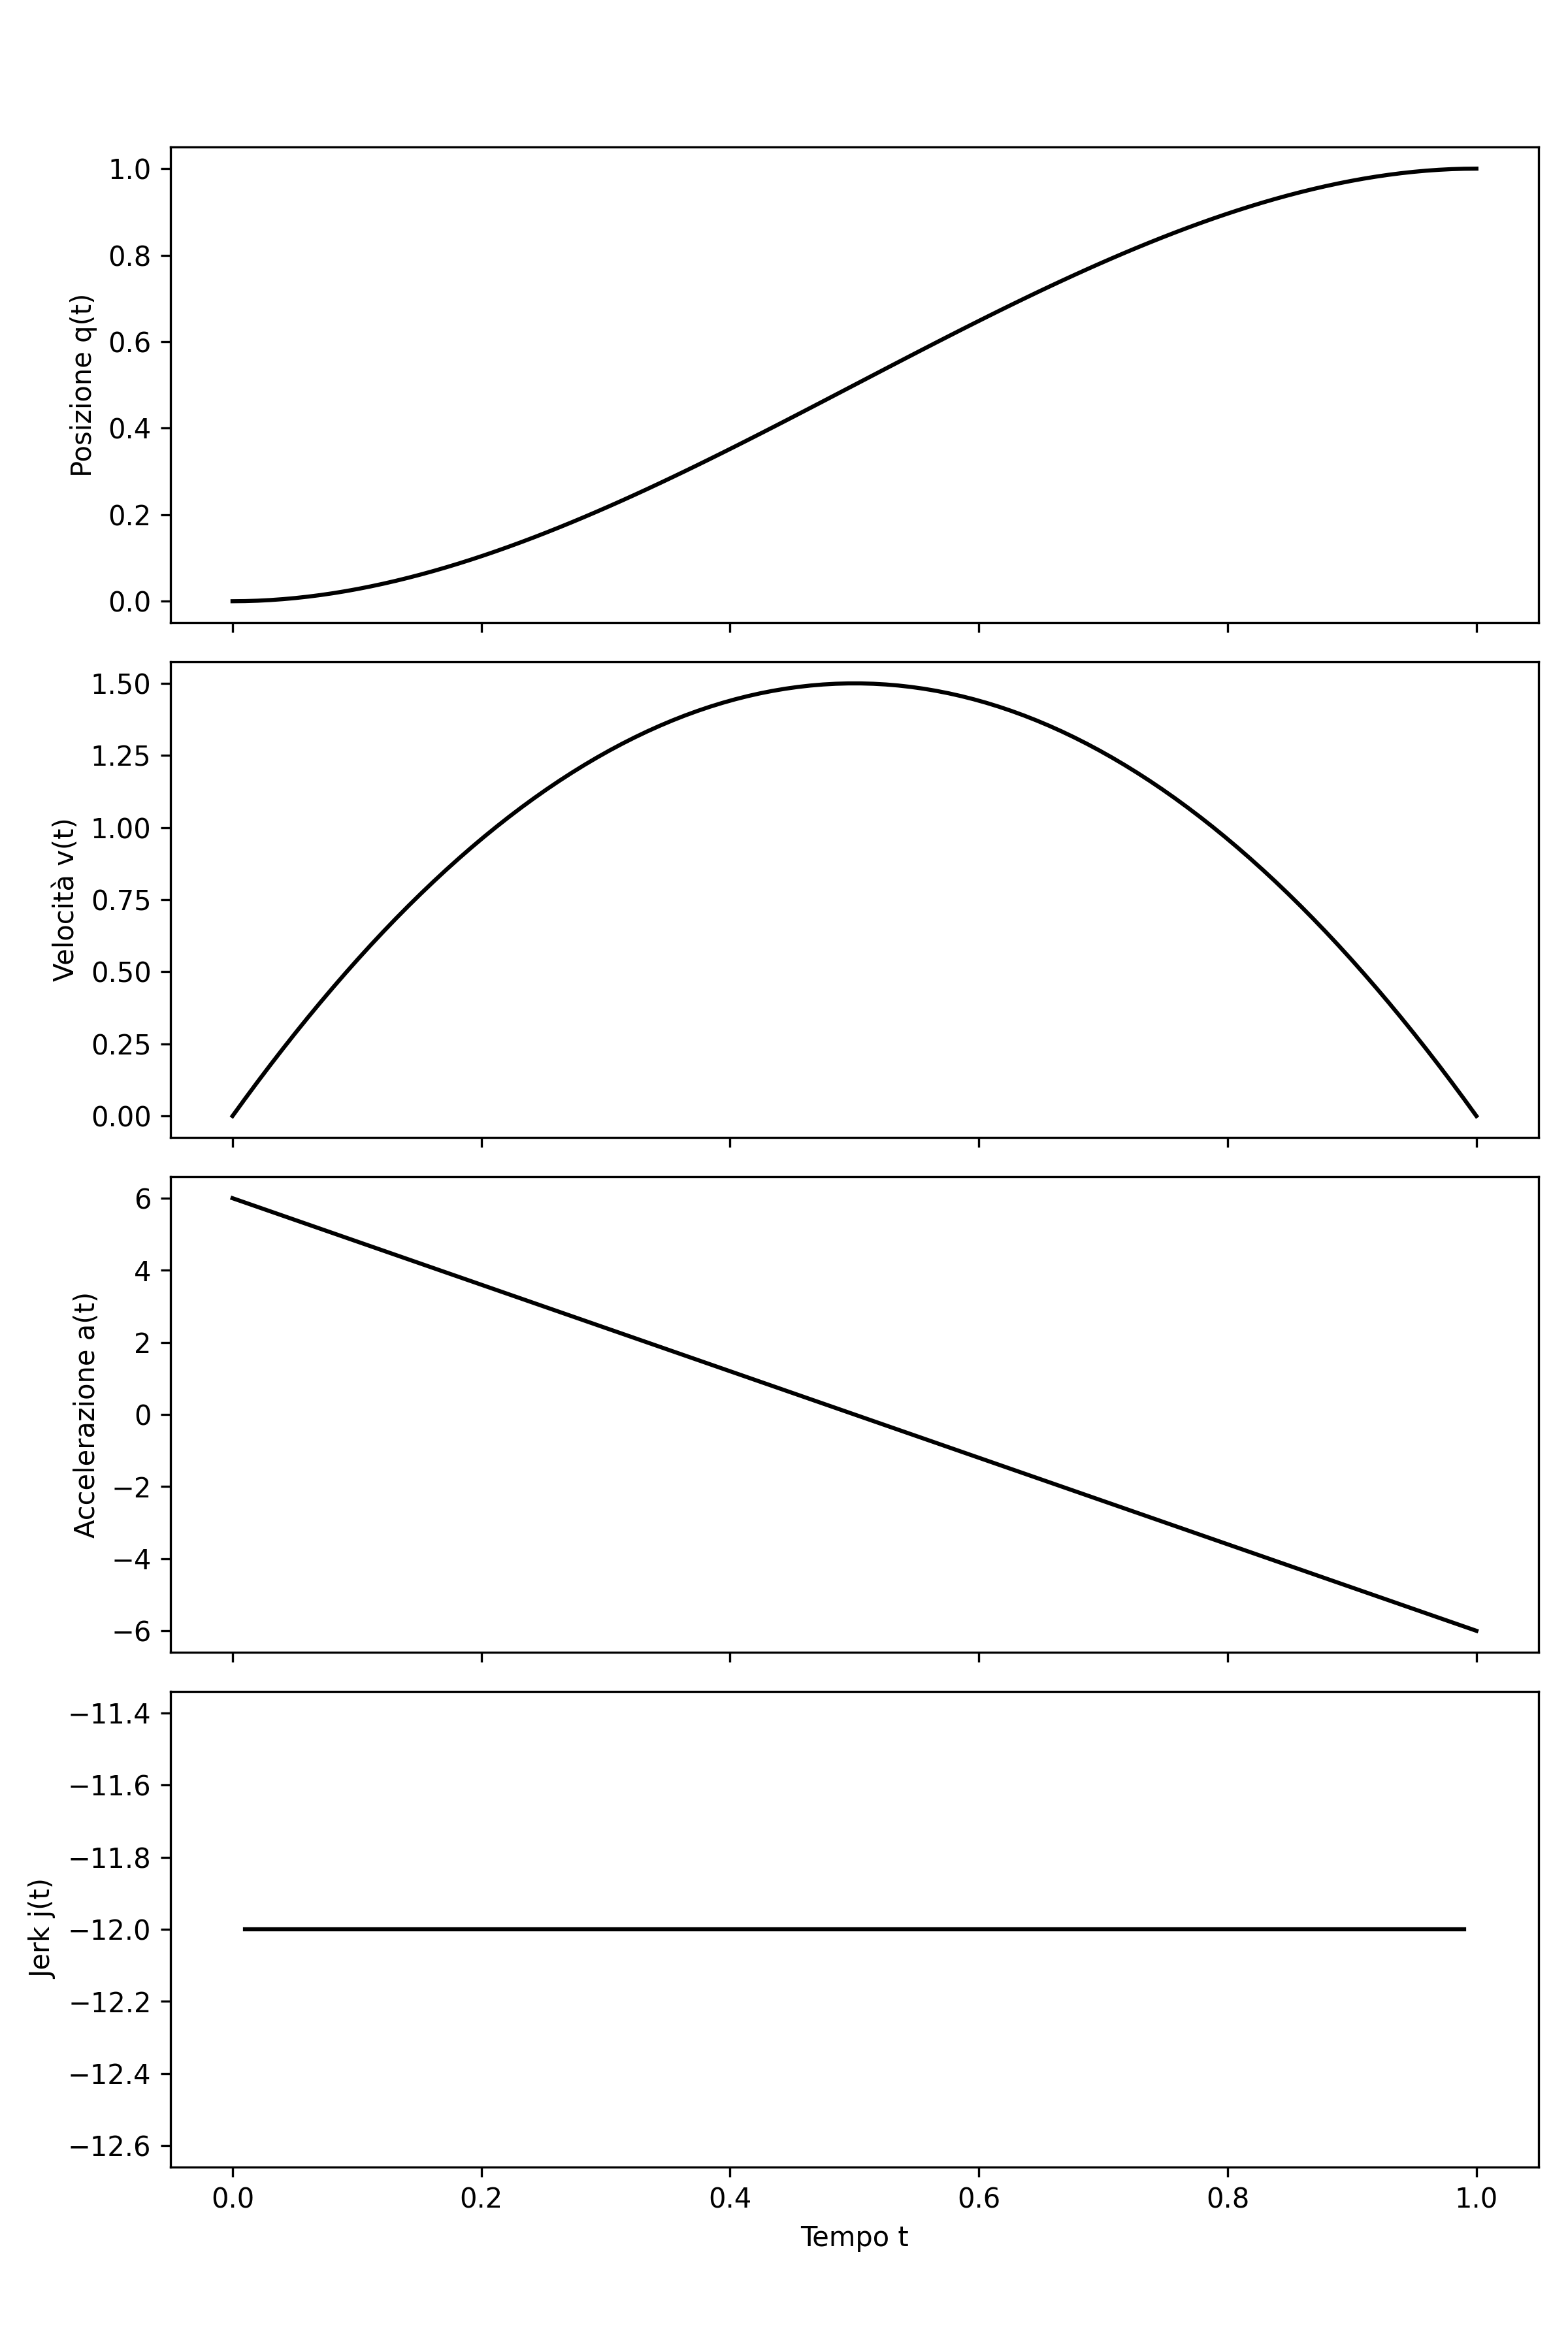
\includegraphics[width=0.3\textwidth]{Immagini/polinom_terzo_grado.png}
    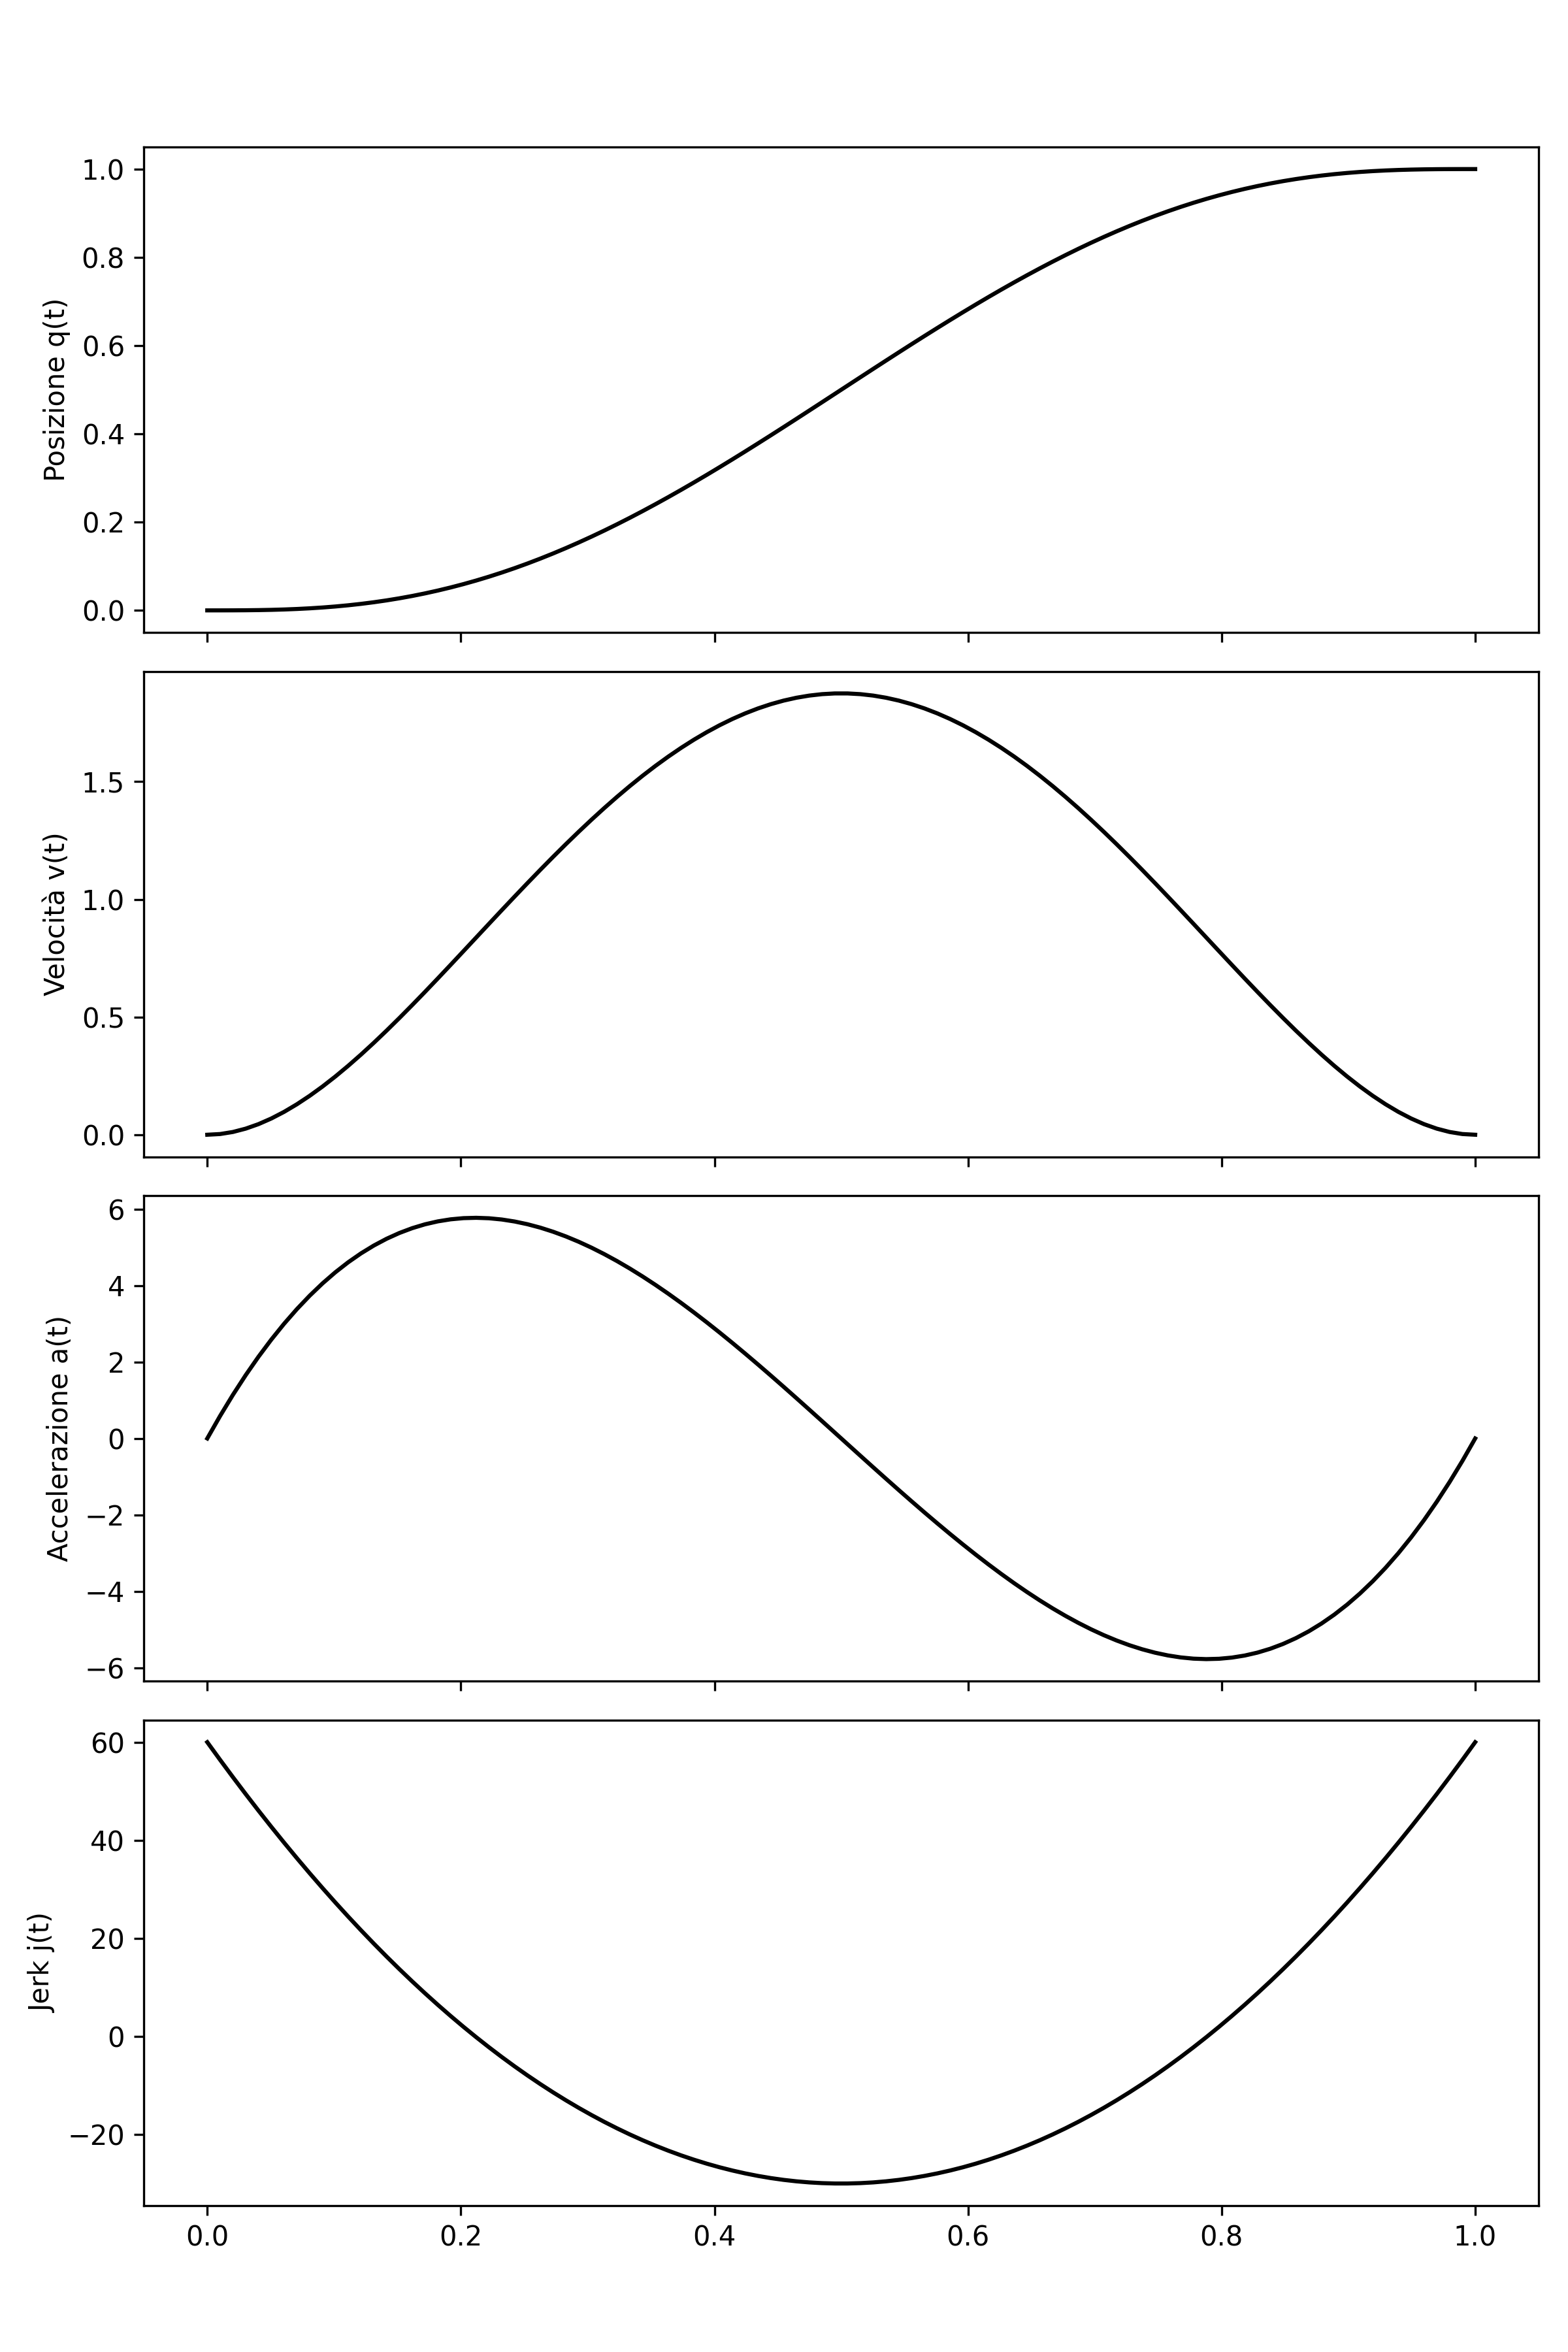
\includegraphics[width=0.3\textwidth]{Immagini/polinom_quinto_grado.png}
    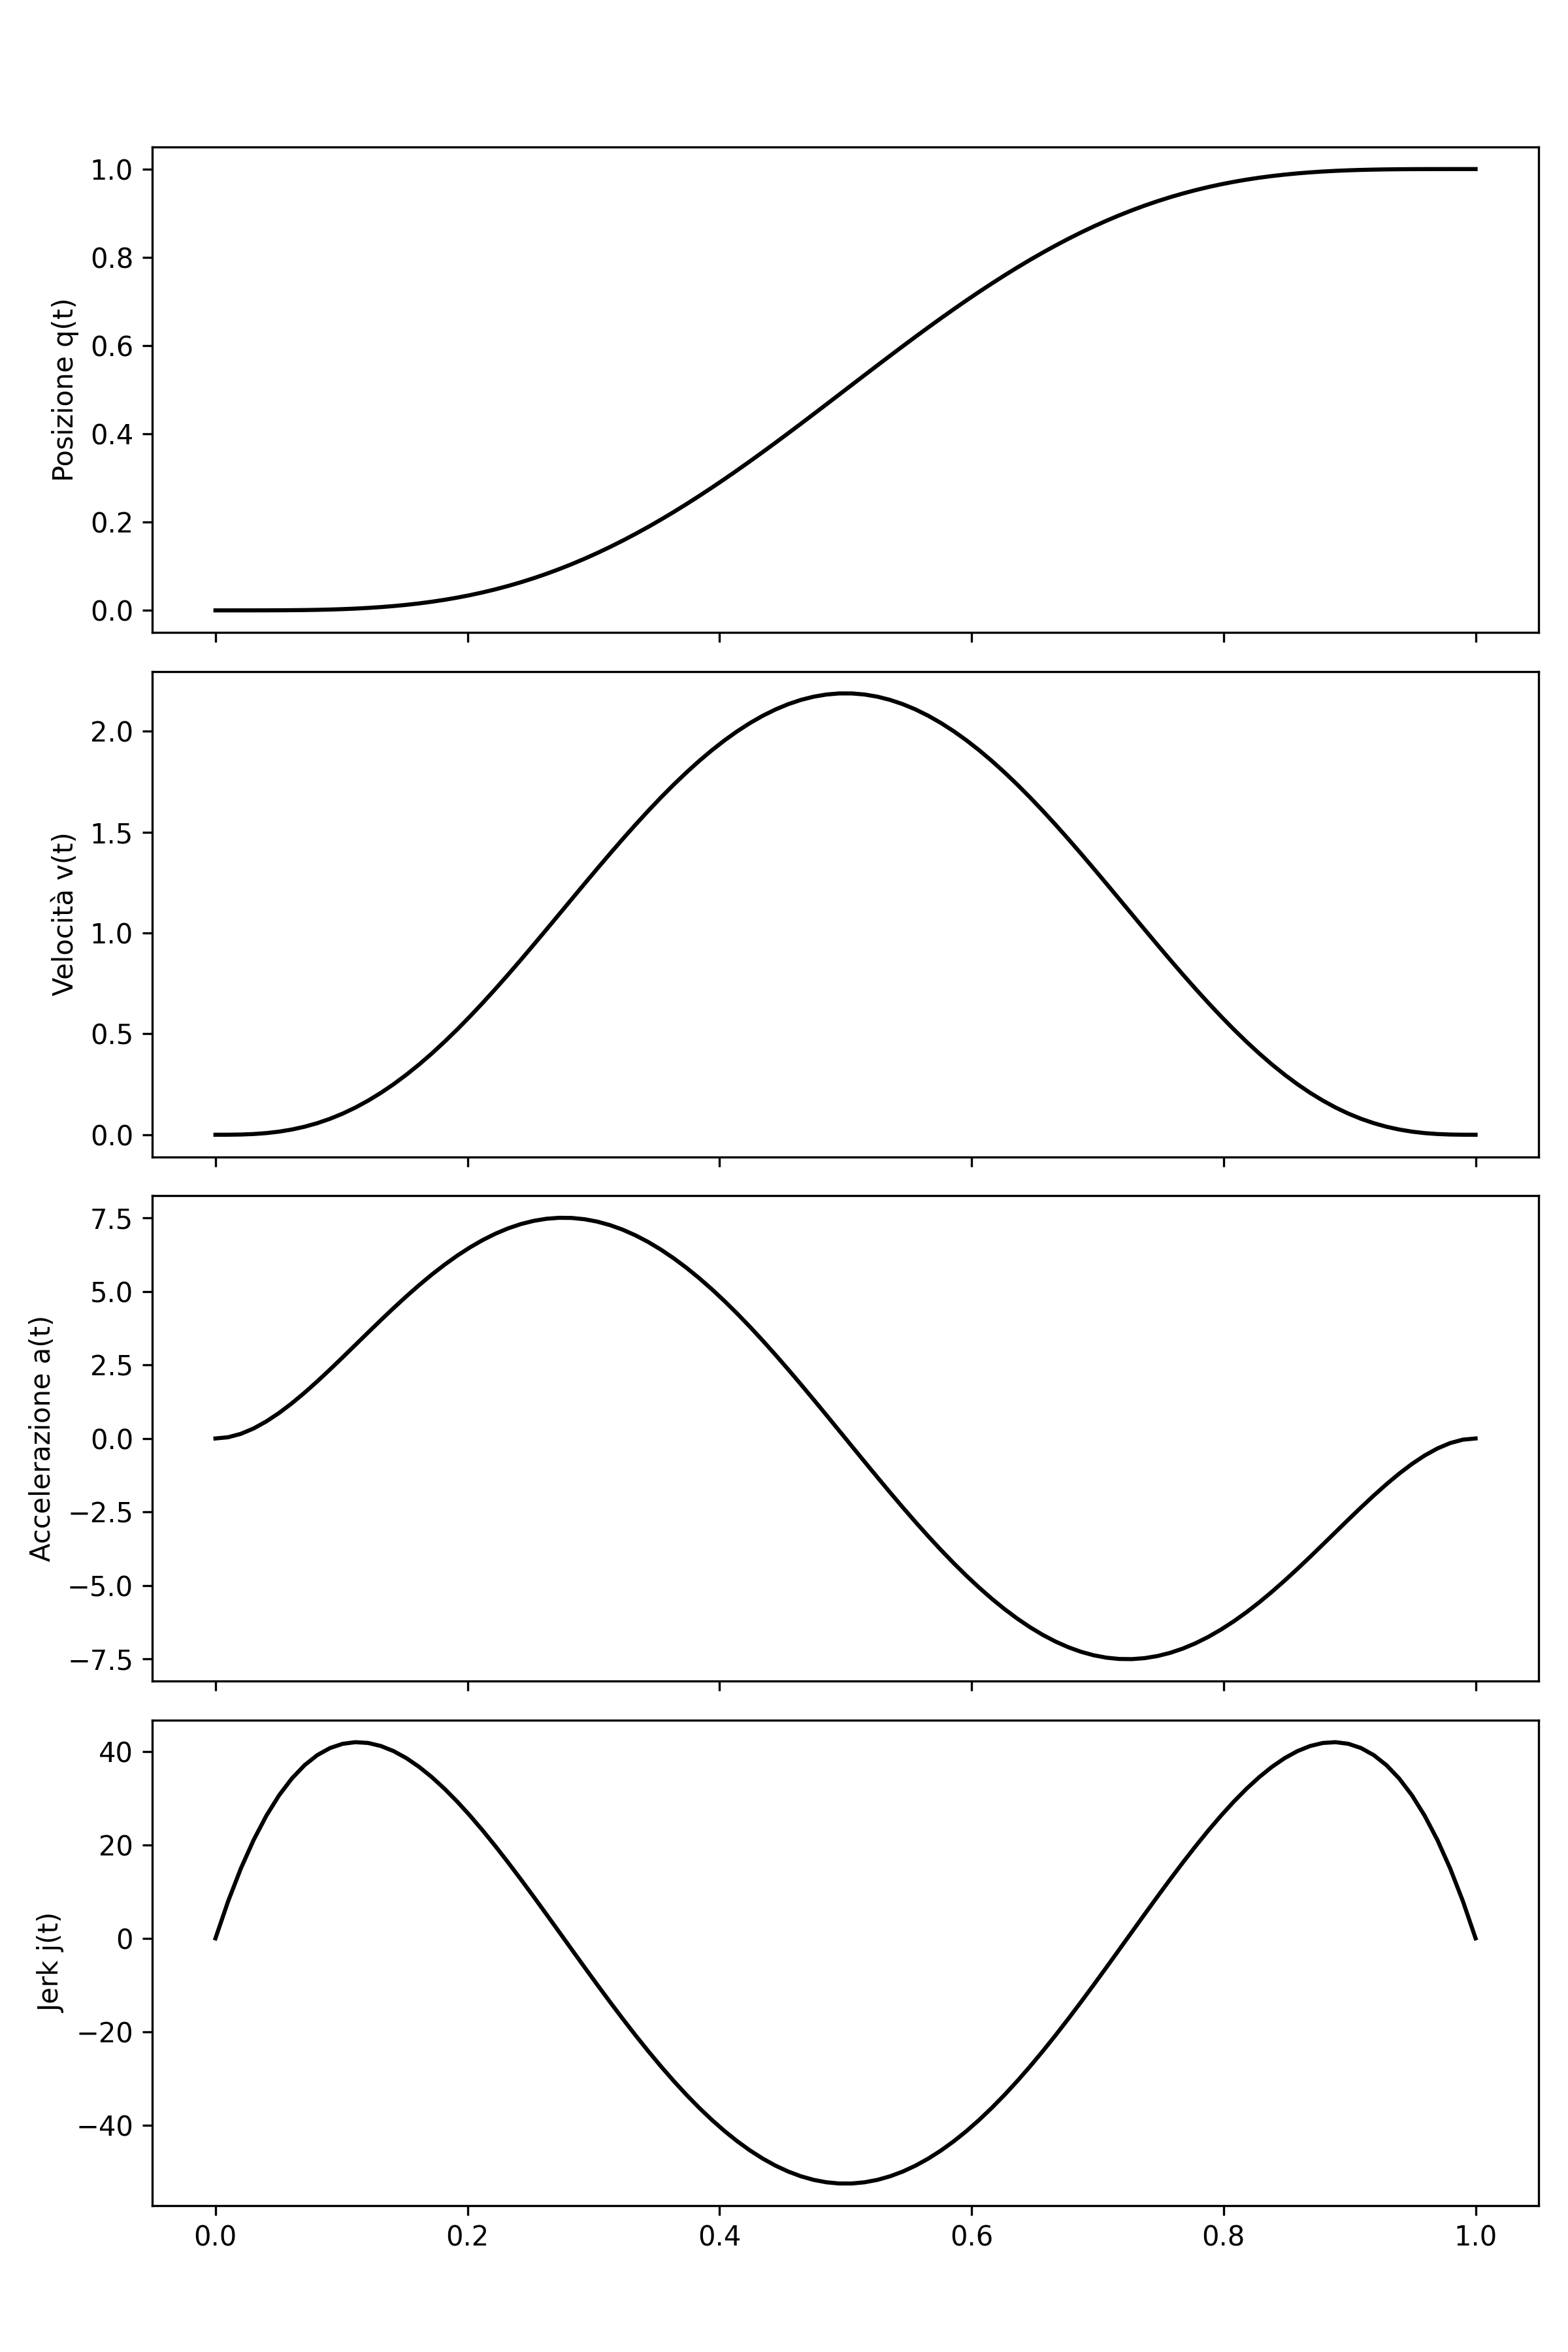
\includegraphics[width=0.3\textwidth]{Immagini/polinom_settimo_grado.png}
    \caption{Polinomiali (RtR) grado 3 (sx), 5 (centro), 7 (dx)}
\end{figure}

\sottosezione{Leggi Trigonometriche}
Quando nelle leggi vengono utilizzati seni e coseni. I risultati sono molto comparabili con leggi polinomiali.
Sono definite in RtR, possono essere però adattate per condizioni iniziali e finali differenti.

\paragrafo{Cicloidale:}
La legge cicloidale o sinusoidale in accelerazione è una legge molto dolce, che però ha coefficienti di velocità e accelerazione alti. Risulta paragonabile con la polinomiale di quinto grado.

\paragrafo{Armonica:}
La legge armonica viene definita come mezzo periodo di una legge cosinusoidale, in velocità e accelerazione ha valori buoni. In particolare rispetto la polinomiale di terzo grado vede un miglioramento dell'accelerazione massima, che risulta nuovamente all'istante iniziale.

\sottoparagrafo{Raccordi:}
A partire dalla legge armonica, che risente della ridotta dolcezza legata al jerk infinito, è possibile modificare la legge introducendo un raccordo sinusoidale\footnote{I raccordi tendenzialmente non sono lineari. La durata del raccordo in applicazioni pratiche è T/8.}

\sezione{Composizione di Leggi di Moto}
In modo simile a come fatto per i raccordi, è possibile a partire da specifiche di progetto, comporre diverse leggi di moto. Per semplicità di formulazione in casi generici si utilizzano leggi polinomiali almeno in prima istanza (sarebbe più complicato determinare condizioni iniziali di velocità e accelerazione non nulle per leggi più complesse).

Per la corretta formulazione occorre seguire i seguenti step:
\begin{enumerate}
    \item Scrivere esplicitamente le condizioni
    \item Contare le condizioni
    \item Identificare il grado del polinomio (in relazione al numero di condizioni)
    \item Calcolo dei coefficienti del sistema
\end{enumerate}

\paragrafo{Disaccoppiamento}
Potrebbe essere possibile risolvere i sotto-problemi separatamente se sono disaccoppiati tra loro.
Non è vero in generale, perchè i sotto-problemi possono essere tra loro accoppiati.

\sottosezione{Tratti a Velocità Costante Imposta}
Nell'esempio in figura vengono distinte quattro zone, ciascuna delle quali vede associata una legge di moto.
Questo è uno di quei casi particolari in cui le leggi di moto possono essere ricavate separatamente (per questo nella risoluzione la zona4 viene affrontata prima della zona3).
L'accelerazione, per questo esempio, basta non sia infinita, ossia la velocità dev'essere continua (potrebbe non essere derivabile nel dominio)\footnote{HMW: Capire cosa cambia per accelerazione continua e per accelerazione, jerk continui (tipiche richieste da esame).}.


\paragrafo{Zona 1:}
Condizione di velocità, posizione, per tempi iniziale e finale: \(q(t_0)=P_0, \ q(t_1)=P_1, \ \dot{q}(t_0)=0, \ \dot{q}(t_1)=v \), per \(t\in [t_0,t_1]\); le condizioni sono 4, perciò la polinomiale sarà di terzo grado; a partire dalle condizioni è possibile ricavare i coefficienti della polinomiale.

\paragrafo{Zona 2:}
Tratto a velocità costante: \(q(t)=P_1+v(t-t_1)\), per \(t\in [t_1,t_2]\)

\paragrafo{Zona 4:}
Tratto di sosta\footnote{Attenzione a non complicarsi inutilmente la vita andando a scrivere leggi polinomiali quando basta semplicemente scrivere posizione uguale a costante.}: \(q(t)=P_0\), per \(t\in [t_3,t_4]\).

\paragrafo{Zona 3:}
Tratto di ritorno: condizione di velocità, posizione, per tempi iniziale e finale: \(q(t_2)=P_2, \ q(t_3)=P_0, \ \dot{q}(t_2)=v, \ \dot{q}(t_3)=0 \), per \(t\in [t_2,t_3]\); le condizioni sono 4, perciò la polinomiale sarà di terzo grado.

\sottosottosezione{Tracciamento qualitativo dei grafici}
Per il tracciamento dei grafici conviene partire dalle tangenti nei punti di interesse (inizio, fine, congiungimento a tratti noti). 
Occorre prestare attenzione alle cuspidi in posizione. 
Bisogna fare attente valutazioni sui valori di velocità inziali e finali (in questo caso non sono richiesti a 0), e se sia o meno continua (in questo caso no).
Occorre fare opportune valutazioni sul grafico tracciato in velocità per determinare l'andamento dell'accelerazione che deve necessariamente essere coerente, valutando se sia continua o meno (in questo caso no).

\sottosottosezione{Punto di massimo di posizione}
Nel definire le leggi di moto per i vari tratti è possibile che in posizione vi sia sovraelongazione quando si dovesse avere un'inversione di velocità, ad esempio per ritornare ad un punto iniziale, o comunque precedente. Il problema legato alla sovraelongazione è che non è noto a priori il valore massimo di posizione, nè il tempo cui avviene. Pensando in ottica di ritorno alla posizione di partenza, di solito questa viene effettuata nel minor tempo possibile, portando quindi ad avere nelle peggiori condizioni in termini di velocità e accelerazione, anche un massimo di posizione.

\paragrafo{Scelta punto di inversione:}
Per risolvere questo problema occorre imporre il punto di inversione in termini di tempo e posizione. Fatto ciò si divide la zona in cui è presente l'inversione in due, una prima in cui si arriva fino al massimo e una seconda in cui dal massimo si vada a scendere. In particolare la seconda di queste due zone aggiuntive, noto che l'inversione viene effettuata per velocità nulla (per massimo della funzione posizione), e sempre in condizione di ritorno alla posizione precedente, è nelle condizioni di RtR, per cui è possibile ottimizzare la legge andando a scegliere la legge di moto più adatta all'applicazione.

\paragrafo{Scelta del tempo di inversione:}
La scelta di tempo di inversione è determinato dalla necessità di ridurre le velocità e accelerazioni massime e RMS, cosa fattibile per le valutazioni sulla zona che segue il punto di inversione. C'è tuttavia da notare che per la zona precedente il punto di inversione, invece, non è detto ci sia una condizione tanto favorevole, per tempi lunghi e polinomiali di grado elevato potrei avere l'insorgere di massimi/minimi relativi/assoluti in prossimità della posizione di inversione. Per scongiurare quest'evenienza è sufficiente limitare il tempo di posizione di inversione, oltre a questo limitare il tempo di sovraelongazione permette di dedicare più tempo alla discesa.

\sottosezione{Passaggio Esatto per N Punti Intermedi}
Per la risoluzione di un problema in cui sia richiesto il passaggio esatto per un numero di punti intermedi si utilizza il metodo \textbf{S.P.Line}, Smooth Path Line, per via dell'accelerazione continua che viene richiesta, quindi perché la legge è dolce.

\sottosottosezione{Condizioni}
Per la posizione sono definite dalle specifiche del problema, per N punti sono \(2(N-1)\) condizioni. Per la velocità è richiesta la continuità per punti intermedi, perciò le leggi \(i, \ i+1\) devono necessariamente avere rispettivamente velocità finale e iniziale uguali \(\dot{q}_i(t_{i+1})=\dot{q}_{i+1}(t_{i+1})\) (il problema è accoppiato perché non sono noti i valori intermedi di velocità), le condizioni sono \(N-2\). Sono inoltre necessarie le condizioni iniziali e finali di velocità, sono quindi 2 condizioni. Per l'accelerazione è richiesta continuità nei punti intermedi quindi le leggi \(i, \ i+1\) devono avere rispettivamente accelerazioni finali e iniziali uguali \(\Ddot{q}_i(t_{i+1})=\Ddot{q}_{i+1}(t_{i+1})\), sono quindi \(N-2\) condizioni.
Sommando tutto si ottengono \(4(N-1)\) condizioni, ciò significa che avrò \(N-1\) polinomi di grado 3. 

\begin{figure}[h]
    \centering
    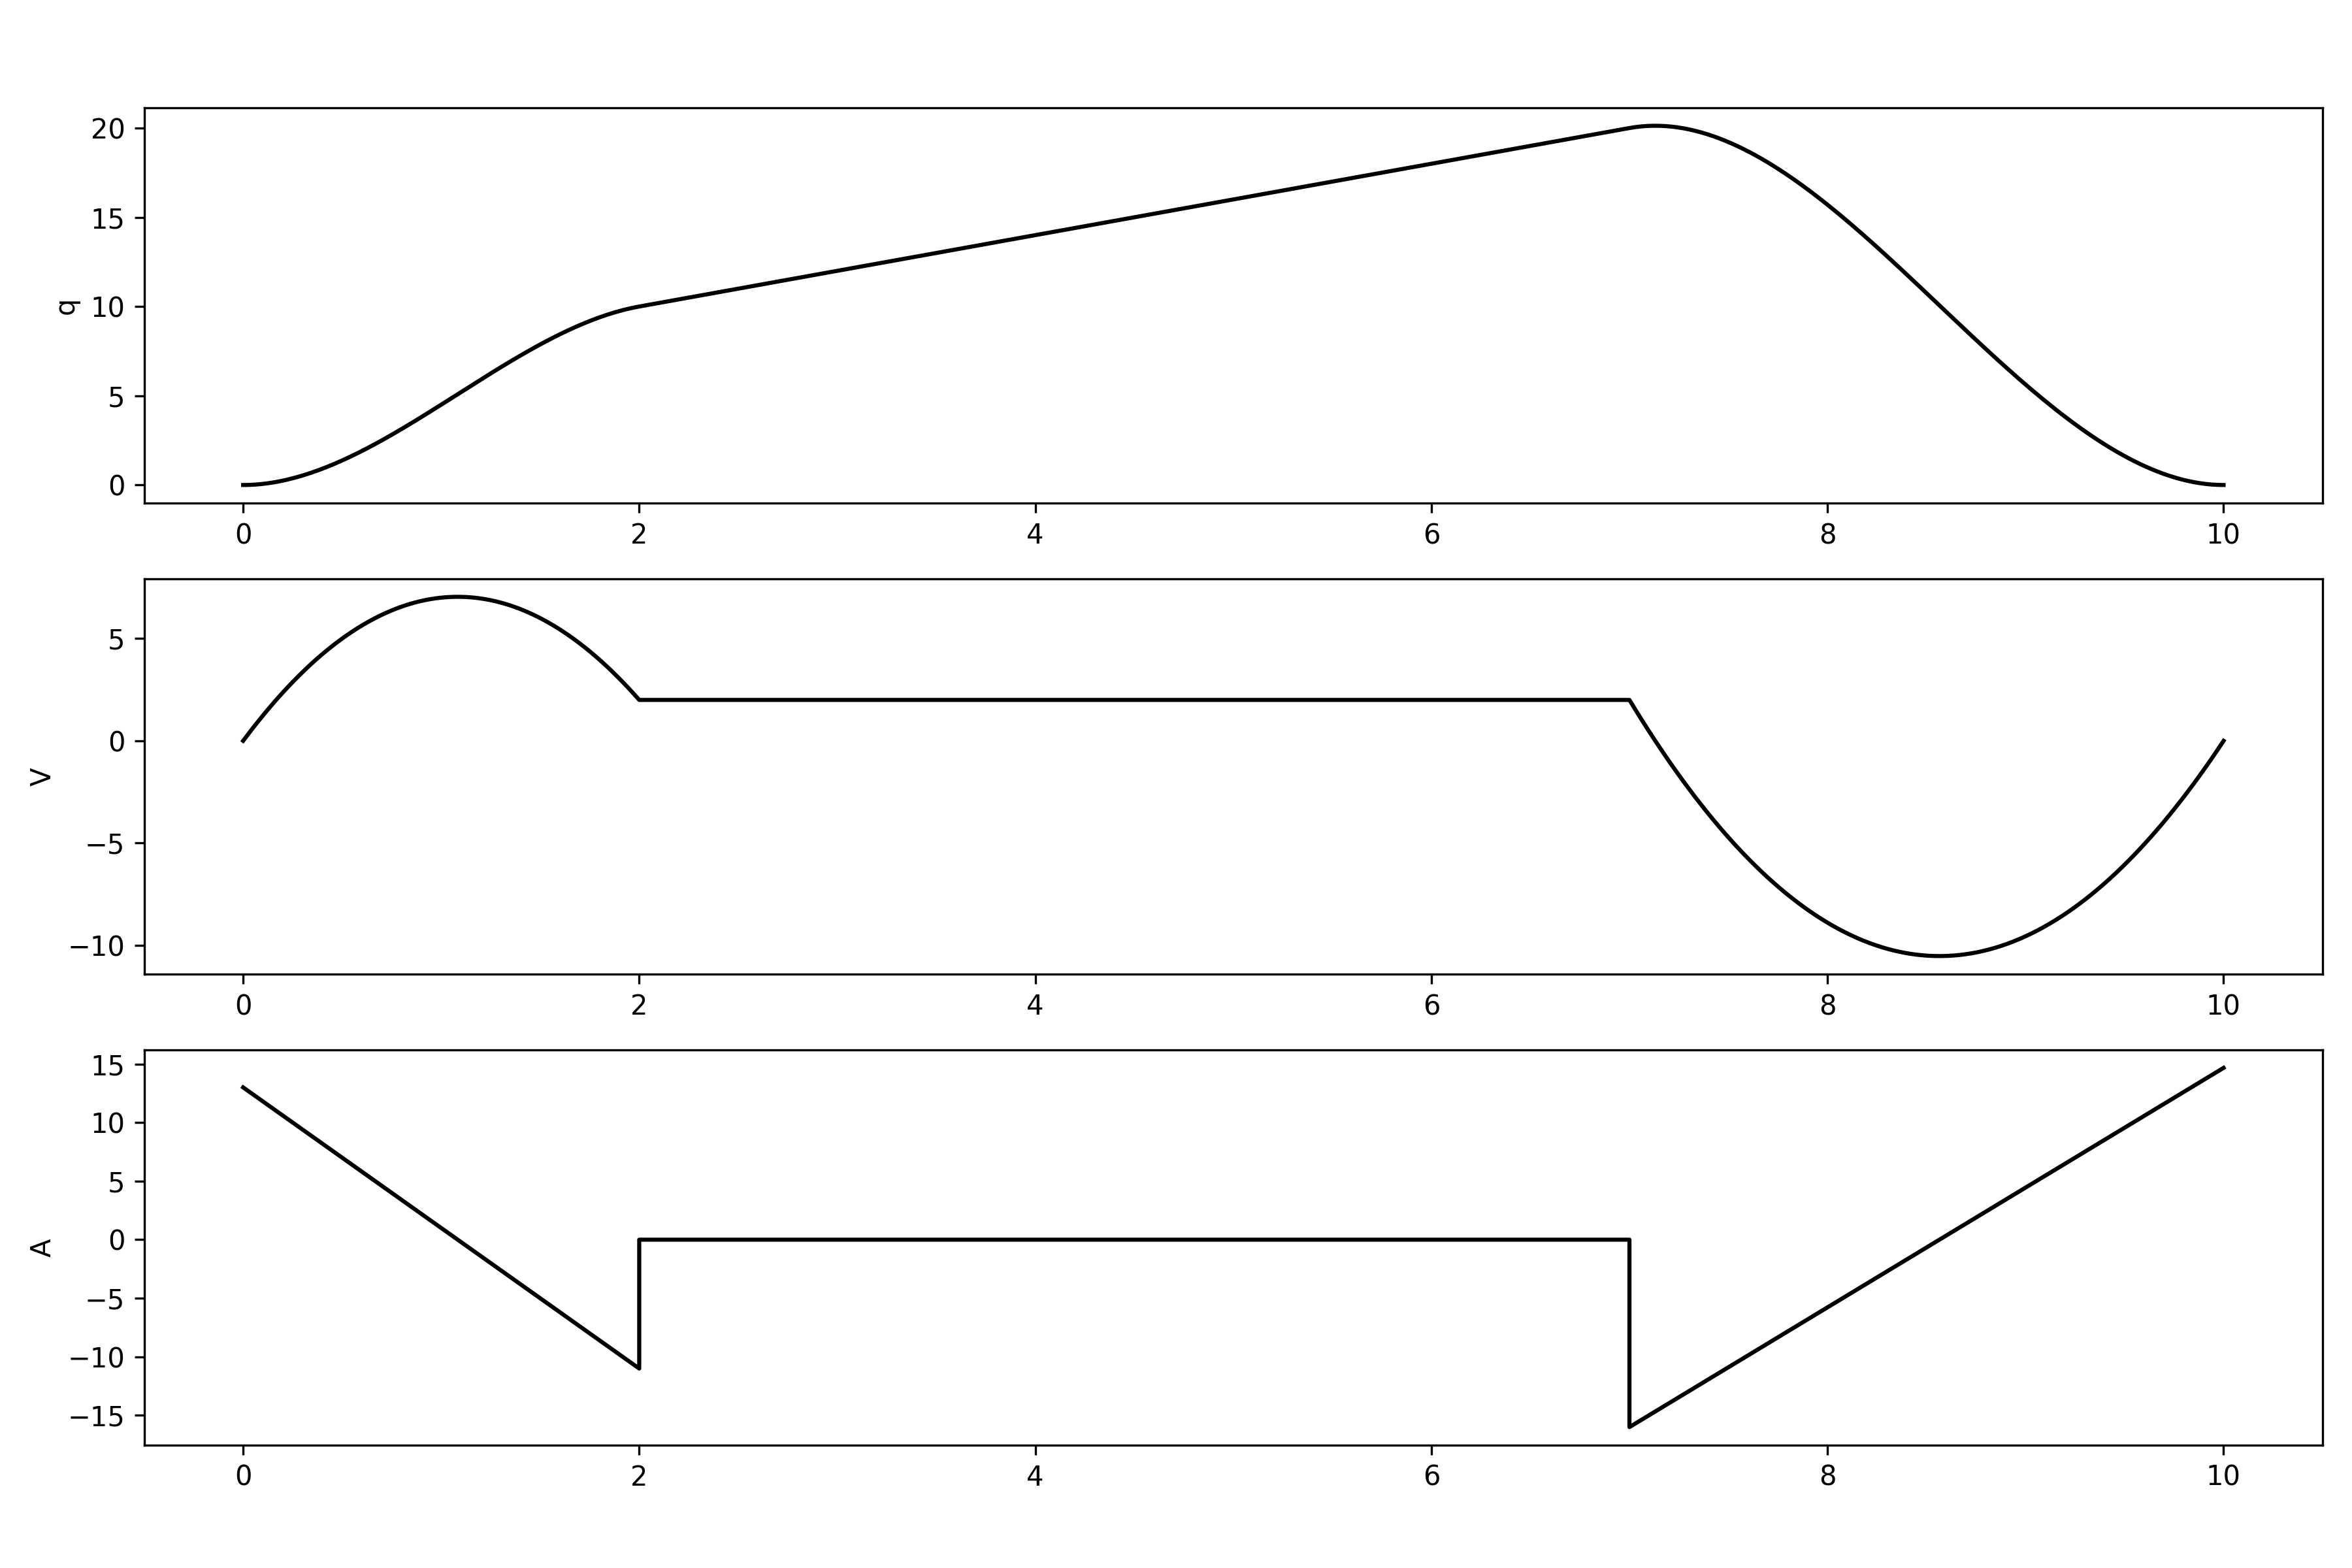
\includegraphics[width=0.6\textwidth]{Immagini/tratti_vel_cost.png}
    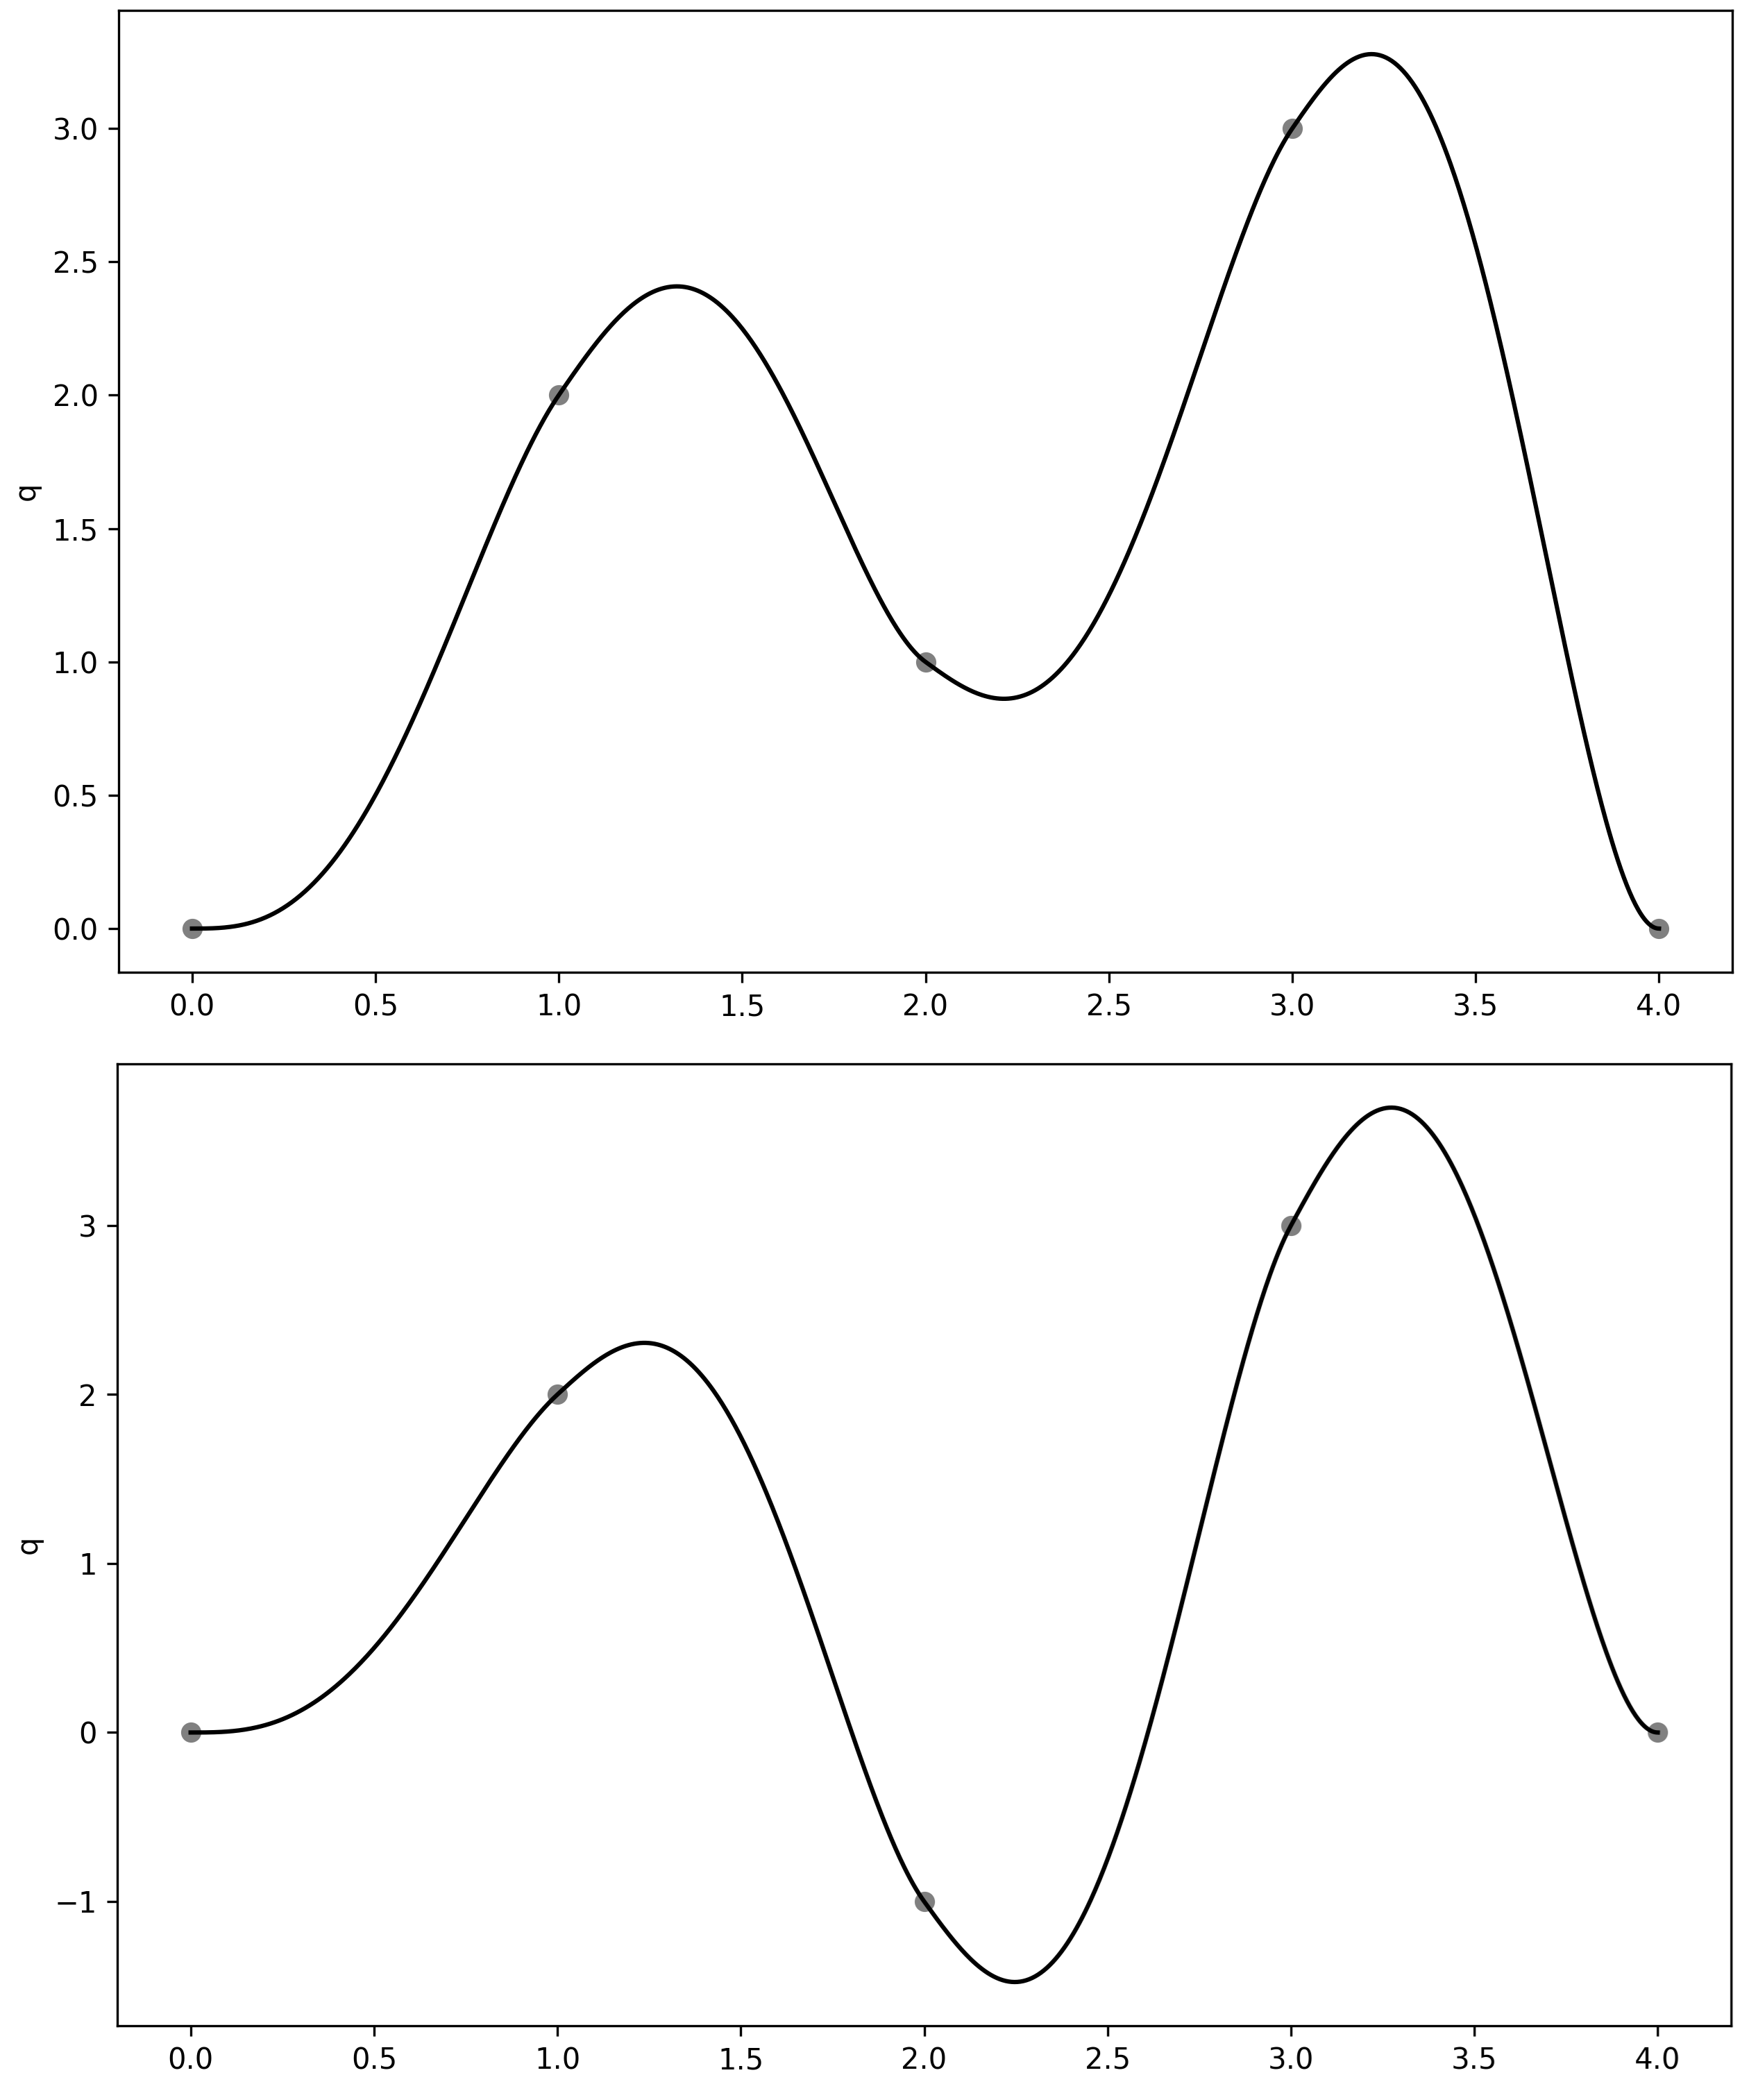
\includegraphics[width=0.3\textwidth]{Immagini/SPLine_spostamento_punto.png}
    \caption{Es tratti a velocità costanti (sx); Spostamento punto SPLine (dx)}
\end{figure}

\sottosottosezione{Soluzione}
Per risolvere il problema è necessario esplicitare TUTTE le condizioni, questo perché in velocità e accelerazione ci sono accoppiamenti tra le singole leggi polinomiali.
Così facendo viene evidenziato il sistema lineare, che è facile da risolvere:
\[ 
\begin{bmatrix}
... \\ ::: \\ ::: \\ ::: \\ ::: \\ ::: \\ :::
\end{bmatrix} 
\begin{Bmatrix}
    a_{0,i} \\ a_{1,i} \\ a_{2,i} \\ a_{3,i} \\ : \\ : \\ a_{3,n-1}
\end{Bmatrix} =
\begin{Bmatrix}
    \text{Termini} \\ \text{Noti} \\ ::: \\ ::: \\ ::: \\ ::: \\ :::
\end{Bmatrix}
\]

\paragrafo{Senso fisico dell'accoppiamento:}
Avere un accoppiamento significa che la matrice di cui sopra non è a blocchi. Significa anche che modificare la posizione o il tempo di un punto va a modificare TUTTI gli altri polinomi.


\sottosezione{SPLine}
La Smooth Path Line permette di creare leggi di moto polinomiali per costruire una legge di moto a partire da specifiche in termini di passaggio obbligato per punti in posizione e tempo.
In generale viene richiesta continuità di posizione e velocità in ogni punto, se poi fosse richiesta continuità di accelerazione unicamente per punti interni si potrà utilizzare una SPLine cubica (perché \(4*N-1\) condizioni).
Se però volessimo imporre accelerazione continua anche nei punti di estremo, ossia \(\Ddot{q}_i(t_1)=A_{in}\) e \(\Ddot{q}_{n-1}(t_n)=A_{fin}\), quindi ci fossero due condizioni aggiuntive, il primo e l'ultimo polinomio dovranno essere di quarto grado; si parla in questo caso di \textbf{SPLine 434} (usata anche in Robotica Industriale).

\paragrafo{Sintesi:}
La SPLine permette di avere una legge dolce, perchè avente jerk finito.
Tuttavia possono essere presenti sovraelongazione in posizione (anche se tendenzialmente limitate perché il grado di SPLine tendenzialmente è ridotto). E non c'è controllo su velocità e accelerazioni massime e RMS.

\sottosottosezione{Soluzioni}
La presenza di sovraelongazioni in posizione può essere critica.
Ci sono diverse possibili soluzioni:
\begin{itemize}
    \item Introduzione di punti intermedi atti a forzare una determinata forma alla legge di moto
    \item Imposizione di velocità e/o accelerazione nulla nel punto di massimo desiderato, andando a spezzare in due la SPLine proprio nel punto di massimo
    \item Spostaento dei tempi, che permette di ridurre sovraelongazione e di modificare velocità e accelerazioni
\end{itemize}

\sottosottosezione{Esempi SPLine con tratti intermedi a velocità imposta}
Nel primo caso vanno utilizzate due SPLine, perché c'è disaccoppiamento dovuto dai tratti a velocità costante centrale e finale. Se per esempio il punto P8 che è anche quello inferiore dovesse avere una sovraelongazione critica, potrei pensare di far terminare lì la SPLine, imporre condizioni finali di velocità, accelerazione nulla e terminare la legge con la RtR preferita.

Nel secondo caso, rimuovere il tratto a velocità imposta finale, fa sì che non vi sia disaccoppiamento, quindi dalla zona di lavoro 3 si prosegue con la zona di lavoro 1, perciò è opportuno fare un'unica SPLine che iniziano e finiscono nel tratto a velocità costante. Anche in questo caso, se guardando la legge vi fossero punti critici per sovraelongazione potrei andare a separare in due SPLine imponendo sul punto critico velocità e accelerazioni nulle.

\begin{figure}[h]
    \centering
    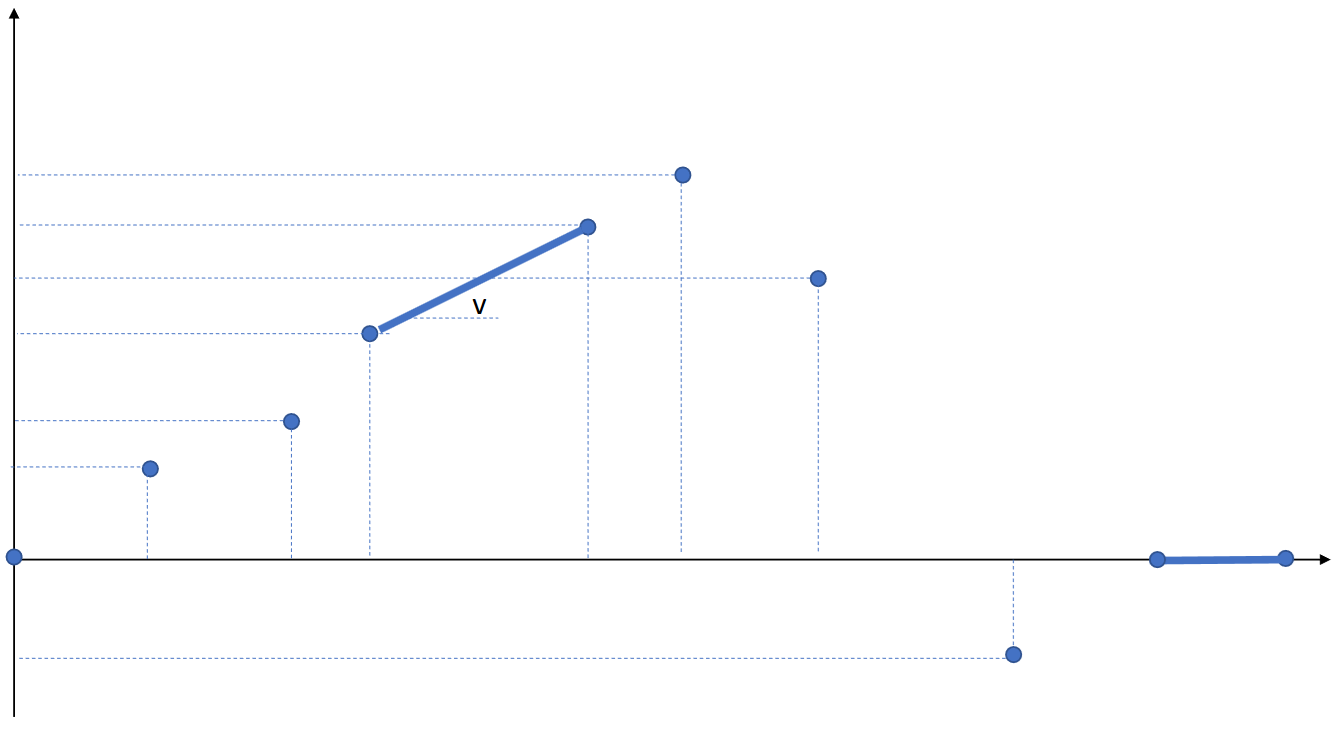
\includegraphics[width=0.4\textwidth]{Immagini/es1_leggi_moto.png}
    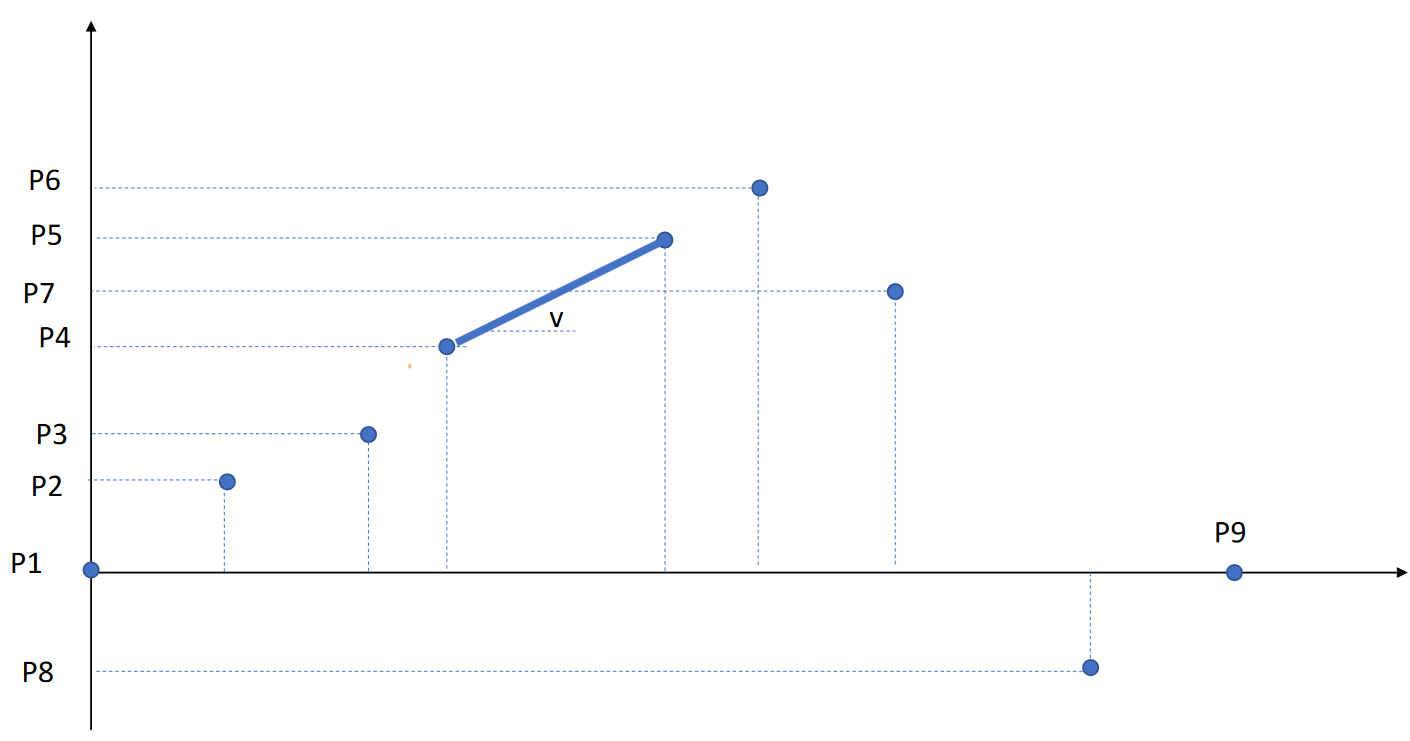
\includegraphics[width=0.4\textwidth]{Immagini/es2_leggi_moto.png}
    \caption{Esercizi 1 sx; 2 dx}
\end{figure}